% This is "sig-alternate.tex" V2.1 April 2013
% This file should be compiled with V2.5 of "sig-alternate.cls" May 2012
%
% This example file demonstrates the use of the 'sig-alternate.cls'
% V2.5 LaTeX2e document class file. It is for those submitting
% articles to ACM Conference Proceedings WHO DO NOT WISH TO
% STRICTLY ADHERE TO THE SIGS (PUBS-BOARD-ENDORSED) STYLE.
% The 'sig-alternate.cls' file will produce a similar-looking,
% albeit, 'tighter' paper resulting in, invariably, fewer pages.
%
% ----------------------------------------------------------------------------------------------------------------
% This .tex file (and associated .cls V2.5) produces:
%       1) The Permission Statement
%       2) The Conference (location) Info information
%       3) The Copyright Line with ACM data
%       4) NO page numbers
%
% as against the acm_proc_article-sp.cls file which
% DOES NOT produce 1) thru' 3) above.
%
% Using 'sig-alternate.cls' you have control, however, from within
% the source .tex file, over both the CopyrightYear
% (defaulted to 200X) and the ACM Copyright Data
% (defaulted to X-XXXXX-XX-X/XX/XX).
% e.g.
% \CopyrightYear{2007} will cause 2007 to appear in the copyright line.
% \crdata{0-12345-67-8/90/12} will cause 0-12345-67-8/90/12 to appear in the copyright line.
%
% ---------------------------------------------------------------------------------------------------------------
% This .tex source is an example which *does* use
% the .bib file (from which the .bbl file % is produced).
% REMEMBER HOWEVER: After having produced the .bbl file,
% and prior to final submission, you *NEED* to 'insert'
% your .bbl file into your source .tex file so as to provide
% ONE 'self-contained' source file.
%
% ================= IF YOU HAVE QUESTIONS =======================
% Questions regarding the SIGS styles, SIGS policies and
% procedures, Conferences etc. should be sent to
% Adrienne Griscti (griscti@acm.org)
%
% Technical questions _only_ to
% Gerald Murray (murray@hq.acm.org)
% ===============================================================
%
% For tracking purposes - this is V2.0 - May 2012

\documentclass{sig-alternate-05-2015}

\usepackage{graphicx}
\usepackage{subcaption}

\begin{document}

% Copyright
%\setcopyright{acmcopyright}
%\setcopyright{acmlicensed}
%\setcopyright{rightsretained}
%\setcopyright{usgov}
%\setcopyright{usgovmixed}
%\setcopyright{cagov}
%\setcopyright{cagovmixed}



\title{B534 Project Final Report: Building Random Forests with Local versus Global Data Distributions}
%
% You need the command \numberofauthors to handle the 'placement
% and alignment' of the authors beneath the title.
%
% For aesthetic reasons, we recommend 'three authors at a time'
% i.e. three 'name/affiliation blocks' be placed beneath the title.
%
% NOTE: You are NOT restricted in how many 'rows' of
% "name/affiliations" may appear. We just ask that you restrict
% the number of 'columns' to three.
%
% Because of the available 'opening page real-estate'
% we ask you to refrain from putting more than six authors
% (two rows with three columns) beneath the article title.
% More than six makes the first-page appear very cluttered indeed.
%
% Use the \alignauthor commands to handle the names
% and affiliations for an 'aesthetic maximum' of six authors.
% Add names, affiliations, addresses for
% the seventh etc. author(s) as the argument for the
% \additionalauthors command.
% These 'additional authors' will be output/set for you
% without further effort on your part as the last section in
% the body of your article BEFORE References or any Appendices.

\numberofauthors{2} %  in this sample file, there are a *total*
% of EIGHT authors. SIX appear on the 'first-page' (for formatting
% reasons) and the remaining two appear in the \additionalauthors section.
%
\author{
% You can go ahead and credit any number of authors here,
% e.g. one 'row of three' or two rows (consisting of one row of three
% and a second row of one, two or three).
%
% The command \alignauthor (no curly braces needed) should
% precede each author name, affiliation/snail-mail address and
% e-mail address. Additionally, tag each line of
% affiliation/address with \affaddr, and tag the
% e-mail address with \email.
%
% 1st. author
\alignauthor
Katherine Metcalf\\
       \affaddr{Department of Computer Science}\\
       \affaddr{Indiana University }\\
       \affaddr{Bloomington, IN, USA}\\
       \email{metcalka@indiana.edu}
% 2nd. author
\alignauthor
Raksha Kumaraswamy\\
       \affaddr{Department of Computer Science}\\
       \affaddr{Indiana University }\\
       \affaddr{Bloomington, IN, USA}\\
       \email{metcalka@indiana.edu}
}

\maketitle
\begin{abstract}
This paper investigates the resilience of Random Forests as classifiers in the distributed data framework. We utilize \textit{Harp} framework as the basic foundation for handling distributed data. We study the performance of Random Forests by varying various properties of this distributed data. We also exploit parallel processing for efficient model in this distributed framework. In conclusion, we provide insightful results into such a modeling framework.
\end{abstract}

\keywords{Random Forests; Distributed data; Harp}

\section{Introduction}
Random Forests \cite{Breiman2001} are a powerful nonparametric statistical class of learning algorithms for both classification and regression tasks. The learned model is a set of trees, where each tree is built by utilizing a bootstrapped random subsample of the training data, hence the name "Random Forests" - a random approach to bootstrap samples, combined with a model that is a set of trees, a forest.

The idea of the algorithm is a simple divide-and-conquer strategy by utilizing bootstrapped samples of the training data - either by subsampling a given bootstrapped sample without replacement and learning a single tree, or by subsampling a given bootstrapped sample with replacement and learning a forest, where for each tree is learned from a subsample pulled from the given bootstrapped data bag. Thus, a Random Forest lends itself naturally to a parallel processing framework for efficient time complexity.

There are many components of the algorithm that can be parallelized. Here are some approaches listed in the order of increasing complexity: (1) generation of the bootstrap samples (with or without replacement), (2) construction of a single tree or forest (and parallelization for the forest construction), based on the sampling procedure used, w.r.t. the bootstrap sample, (3) selection of the decision node during tree construction, etc.

In this paper we present an approach to implementing approaches (1) and (2) above within the \textit{Harp} framework. The focus of our investigation in this paper is to examine how locally versus globally bootstrapping the data bags used to build the trees in the Random Forest impacts the global accuracy of the classifier. This is an important question to address, because data is now collected at a global scale and is stored across the world. Shuffling data around is computationally expensive and vulnerable to security risks while the data is being transported between server locations. Therefore, we investigate the extent to which a globablly shuffling  or model of the data is necessary.

\section{Related Work}
There are many implementations that try to exploit one of the following avenues for parallelization - (1) Ranger - exploits parallelization during feature selection, (2) Map-Reduce Random Forest - where each map job (run in parallel) learns a forest w.r.t the bootstrap sample (sampled with replacement) and the reduce job is just an amalgamation of these various map outputs.

There are also many variations of the basic Random Forests algorithm with different theoretical guarantees and procedures \cite{wright2015ranger,genuer2015random} - (1) map-reduce based Random Forest (as described above) called MR-RF, (2) Bag-of-little bootstrap method (BLB) which aims to ensure the size of MR-RF bootstrap samples is close to \textit{N} (original size of data), but contains at most \textit{m} different datapoints - ensuring coverage of training samples despite random subsampling, without being susceptible to bias (like MR-RF with subsample-size \textit{m} « \textit{n}), (3) strategic sampling methods which help overcome bias inherent to the sub-sampling approaches.

Evaluation for performance of a Random Forest has been done by computing: (1) out-of-bag (OOB) error - evaluates performance of single tree, or a single forest by utilizing samples not used to generate the tree, or forest, and (2) the variable importance, which evaluates the importance of a variable used as the decision node.

\section{Problem Specification}
Our project explores the affect locally bootstrapped data bags versus globally bootstrapped data bags have on the quality of a learned Random Forest classifier. Our experiment therefore addresses a real-world scenario where the data storage is not only distributed across geographical locations, but each data storage "unit" only stores data collected in its designated geographical region. For example, say you have a company like Visa that wants to detect fraudulent instances of credit card activity and that Visa has four data storage locations where each storage location is assigned a geographical region for which it will store user data. Each data storage unit collects customer credit card usage information only for those transactions that take place not used to generate the tree, or forest, within its assigned geographical region. So, the data storage unit facility in North America only contains transaction information for those transactions that take place in the United States, Mexico, and Canada. Due to the distributed nature of the data and the massive scale at which transactions are logged, and then stored at each geographical location, this is a scenario in which the Random Forest classifier must be learned in a distributed way. Ideally, in order to take the greatest advantage of a distributed learning environment, there will be at least one Random Forest learning process for each geographical location such that some proportion of the trees in the overall, global forest are learned on data from each of the geographical locations. However, this set-up could potentially cause a number of problems for the performance of the global Random Forest.

The primary challenge faced when learning a Random Forest classifier in this scenario would be that the prior distributions over the feature values (ie. type of purchase) and over the class labels (ie. fraudulent vs. non-fraudulent) are likely to vary from geographical location to geographical location. This is problematic, because Random Forest assumes that the bootstrapped training data used to learn each tree in the forest is independently and identically distributed (IID) over the global population of data points that the Random Forest will be operating on. This assumption does not hold in the above scenario, because the bootstrapped data points are sampled from a subset of the overall data that is not itself representative of the overall data population. The lack of a global representation at local data instances occurs is because the data points were only generated in a given region of the world making them not identically distributed. The purpose of our project and our experiments is to investigate in what way and the extent to which the violation of this IID assumption impacts the globally learned Random Forest's ability to predict labels for data points that are sampled from the global distribution. The answer to this question is very important, because the cost of incorrectly detecting fraud can be very costly, but so too is the cost of shuffling data points around so that each tree is guaranteed to be learned on an IID bootstrapped sample.

\section{Experiment}
For the purposes of this project, we did not have access to a data set or a computing environment with the characteristics identified above. Therefore, we approximated a similar type of data and computing environment by experimenting with three different sets of eight data subsets from the \textit{PAMAP2} data set, which reflect the characteristics described in the problem specification section above:
\begin{itemize}
\item \textit{Global data} -  features and  labels distributed similarly (data consolidated to global data)
\item \textit{Local-Label data} - the distribution over the labels differ
\item \textit{Local-Feature-Label data} - the distribution over the feature and label values differ between each of the eight subsets
\end{itemize} 
In each of the three cases above, eight \textit{Mappers} were used to simulate different geographical regions. In addition, we contrast these results with models learned by utilizing only 2 of the ``geographical locations", in order to show the comparison between \textit{Truly Global models} , and \textit{Approximate Global models}, where in the case of the latter experiments, only data from 2 locations and 2 \textit{Mappers} were utilized for the last 2 scenarios listed above \textit{Local-Label} and \textit{Local-Feature-Label}().

An overview of this experimental configuration for \textit{Global data} is given in Figure \ref{fig:globalData}, and in Figure \ref{fig:localData} for the other 2 \textit{Local data} configurations.

\begin{figure*}
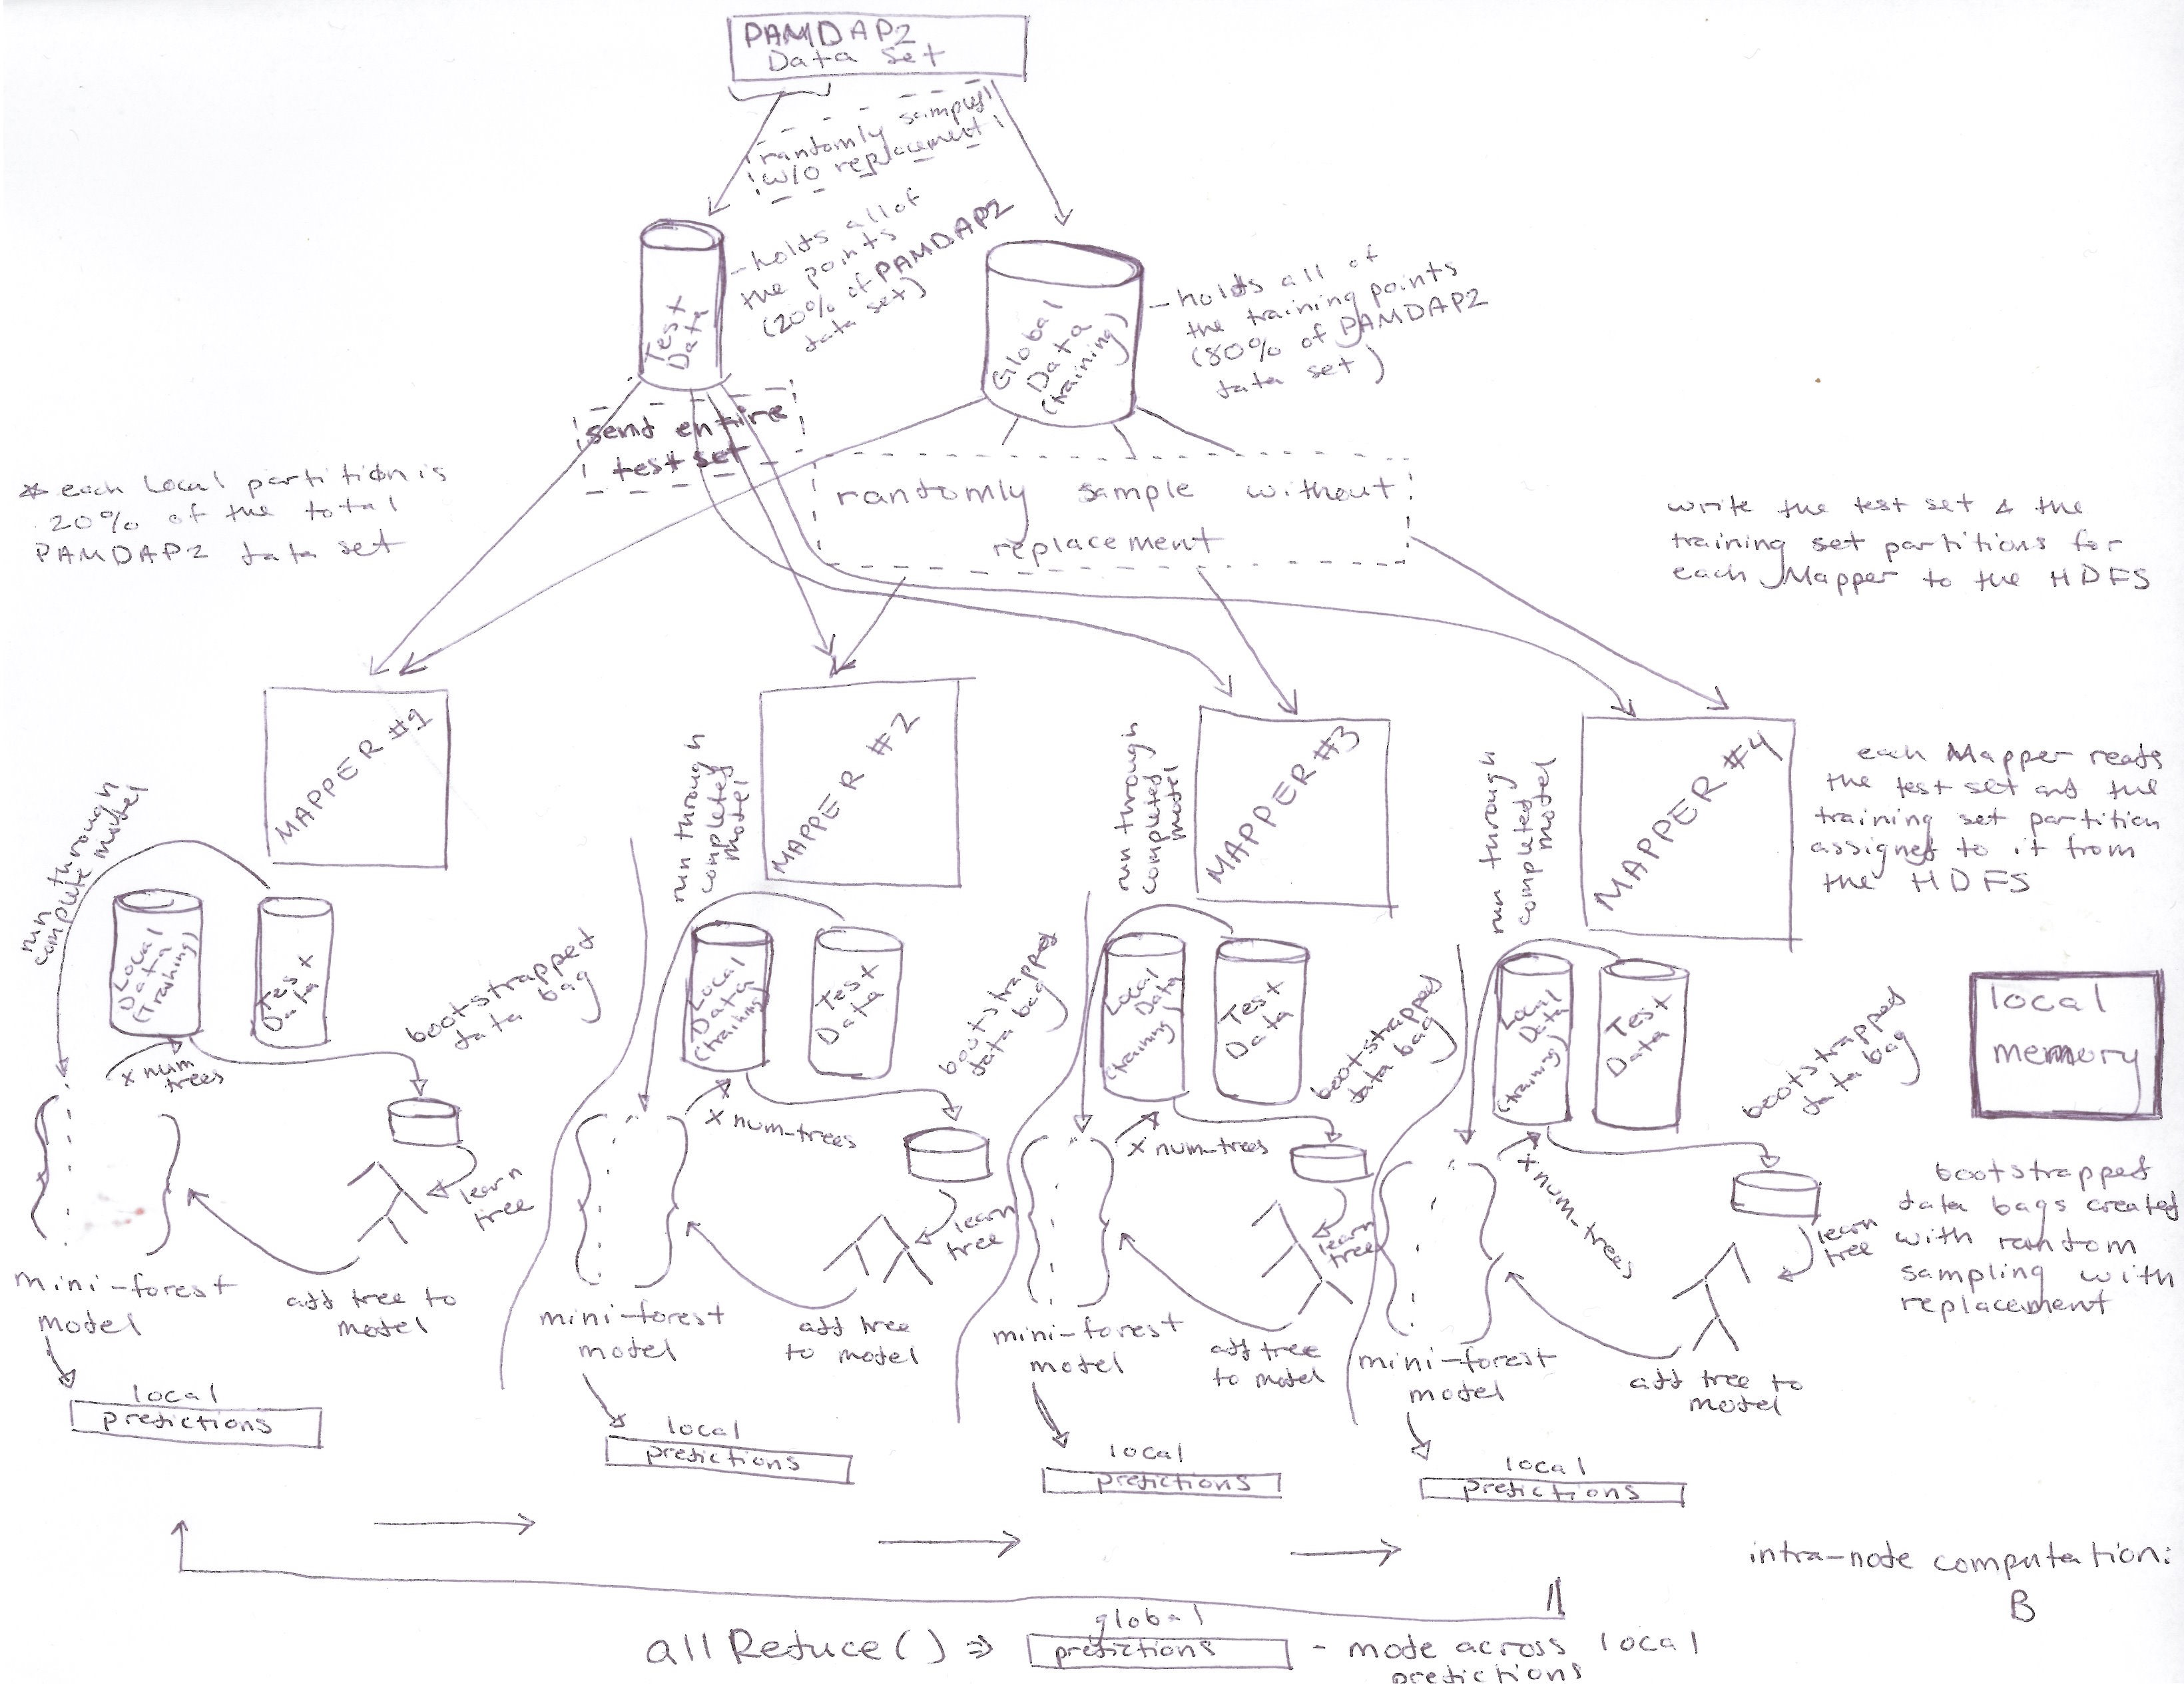
\includegraphics[scale=0.19,angle=90]{figures/globalData.jpg}
\centering
\caption{Overview of the experimental setup and implementation in the case of \textit{Global Data} models. For  representational purposes we show 4 ``geographical location" (4 mappers).}
\label{fig:globalData}
\end{figure*}

\begin{figure*}
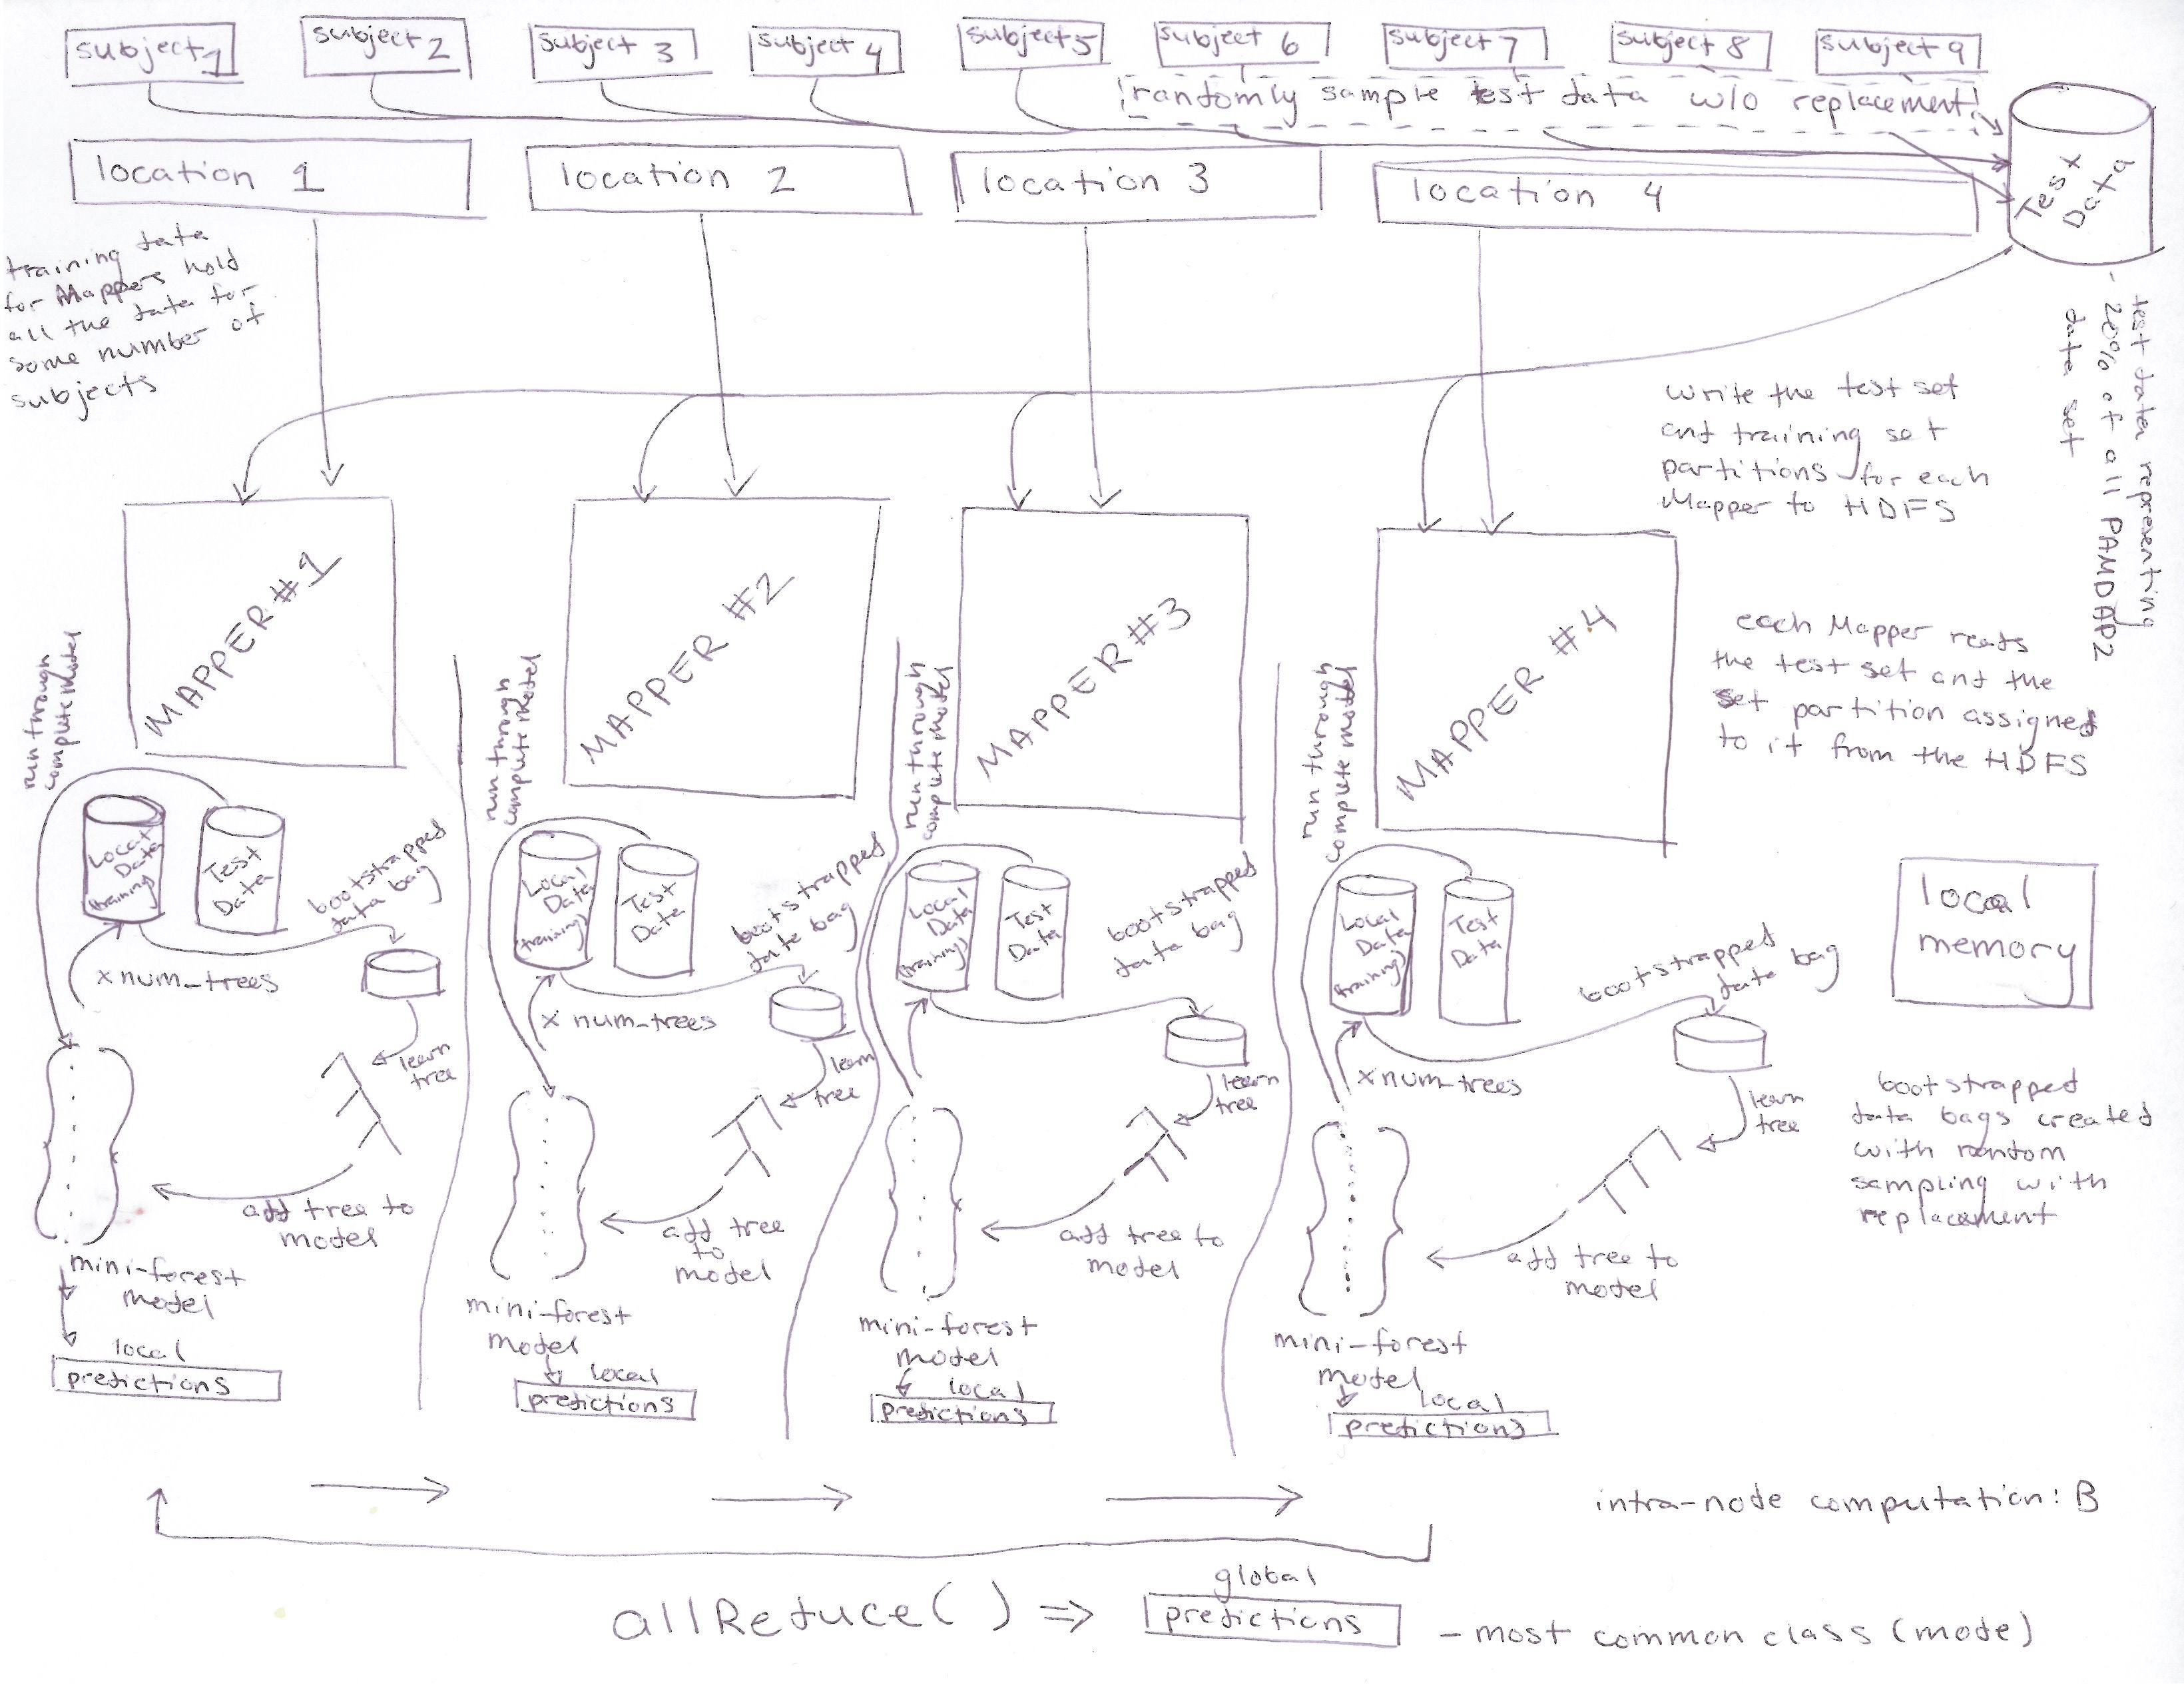
\includegraphics[scale=0.19,angle=90]{figures/localData.jpg}
\centering
\caption{Overview of the experimental setup and implementation in the case of \textit{Local-label data}, and \textit{Local-Feature-Label data} models. For  representational purposes we show 4 ``geographical location" (4 mappers).}
\label{fig:localData}
\end{figure*}

\subsection{Dataset}
The PAMAP2 data set is a multivariate, time-series data set that consists of nine different people who wore three IMU sensors (on their chest, hand, and ankle) and a heart rate monitor while completing a subset of 18 different activities (walking, cycling, playing soccer, etc.). Each participant completed 12 of the possible 18 activities. The PAMAP2 data set consists of the IMU and HR monitor's raw sensory data (sampled every 0.1 seconds) labeled according to the participant the sensory data came from and the type of activity the person was completing at the time. The data set was collected for the purpose of building classifiers that are able to do activity recognition and for investigation into the best ways to do feature selection and feature representation. The feature set consists of 54 real-valued features with 3,850,505 data point instances across participants. For some of the data points the heart rate of the person completing the activity is missing. These data points were excluded for the purpose of this project while utilizing performing the \textit{Approximate Global models} experiment as we did not want any of the limited data in this case to be ``unusable" (essentially, due to missing features). But they were utilized completely in the \textit{Truly Global models}. Given this, in the case of \textit{Approximated Global models}, the size of the dataset for: (1) \textit{Local-label data} - 1 million, and (2) \textit{Local-Feature-Label data} - 658 thousand. The complete dataset (minus the randomly subsampled without replacement test-set) was utilized for the \textit{Truly Global models} experiment. For both the scenarios, we utilized the complete dataset for the \textit{Global data} because: (1) it would be true to the definition, and (2) gives us insight into how Random Forests' performance changes with an increase in the number of trees. The number of treees in a forest are increased by increasing the number of trees each \textit{Mapper} learns within its mini-forest. For example, given a Raondom Forest wher ehte number of trees parameter is set to 100, when the forest is learned with eight \textit{Mappers} it consists of 800 trees and when learned with 2 \textit{Mappers} consists of 200 trees. 

\subsection{Random Forests: Sequential Code}
To aid us in our experiment, we start with an open-source implementation of a Random Forest classifier and incorporate it into the \textit{Harp} framework.  We are utilzing the sequential code provided by \textit{Java ML Library}'s \cite{abeel2009java} open source implementation of the Random Forest algorithm. This code is optimized for fast learning of Random forests with continuous and categorical features. We ran some preliminary experiments with \cite{abeel200java} sequential code on the \textit{PAMAP2} \cite{reiss2012introducing,reiss2012creating} (described in detail in the Experiments section). In \textit{PAMAP2} domain, accuracy of the problem task (predicting activities from the dataset) improved as the number of trees was increased. However, the accuracy difference between 1 tree (22\%) and 50 trees (38\%) is 16\%. Given this poor performance of the learning framework for the 18-way classification problem, we simplify the problem to a binary classification task. We do this as we are interested in studying the effect of the different data distributions on the performance of random forests, and the powerful advantage of utilizing a distributed framework for this task. This analysis will be beneficial when the models learned have a good performance as a baseline to be compared against and this is achieved by making the task simpler; this shifts the focus to distribution of data and it's impact on performance, enabling us to actually compare models. With the task being simplified to a binary task, the sequential code's models have a good performance. Some preliminary results from this experiment are given in Figure !!!. As can be seen, the time taken by the sequential code increases linearly, and therefore we cap the number of trees at 50 in this case. With this \textit{achievable, realistic} performance of the algorithm on this data, we compare various data configurations, its impact on performance, and the pros and cons offered by a distributed parallel framework. 

\subsection{Dataset}
The PAMAP2 data set is a multivariate, time-series data set that consists of nine different people who wore three IMU sensors (on their chest, hand, and ankle) and a heart rate monitor while completing a subset of 18 different activities (walking, cycling, playing soccer, etc.). Each participant completed 12 of the possible 18 activities. The PAMAP2 data set consists of this raw sensory data (sampled every 0.1 seconds) labeled according to the participant the sensory data came from and the type of activity the person was completing at the time. The data set was collected for the purpose of building classifiers that are able to do activity recognition and for investigation into the best ways to do feature selection and feature representation. The feature set consists of 54 real-valued features with 3,850,505 data point instances across participants. For some of the data points the heart rate of the person completing the activity is missing. These data points were excluded for the purpose of this project while utilizing performing the \textit{Approximate Global models} experiment as we do not want any of the limited data in this case to be``unusable" (essentially, due to missing features). But they were utilized completely in the \textit{Truly Global models}. Given this, in the case of \textit{Approximated Global models}, the size of the dataset for: (1) \textit{Local-label data} - 1 million, and (2) \textit{Local-Feature-Label data} - 658 thousand. The complete dataset (minus subsampled without replacement test-set) is utilized for the \textit{Truly Global models} experiment. For both the scenarios, we utilize the complete dataset for the \textit{Global data} because: (1) it would be true to the definition, and (2) it would give us insight into how Random Forests' performance changes with increase in number of trees (with the same data -- this would happen as essentially 8 mappers would create more trees than 2 mappers, on the same bootstrapped global data).

\begin{figure*}[t]
\centering
\begin{subfigure}{.4\textwidth}
\centering
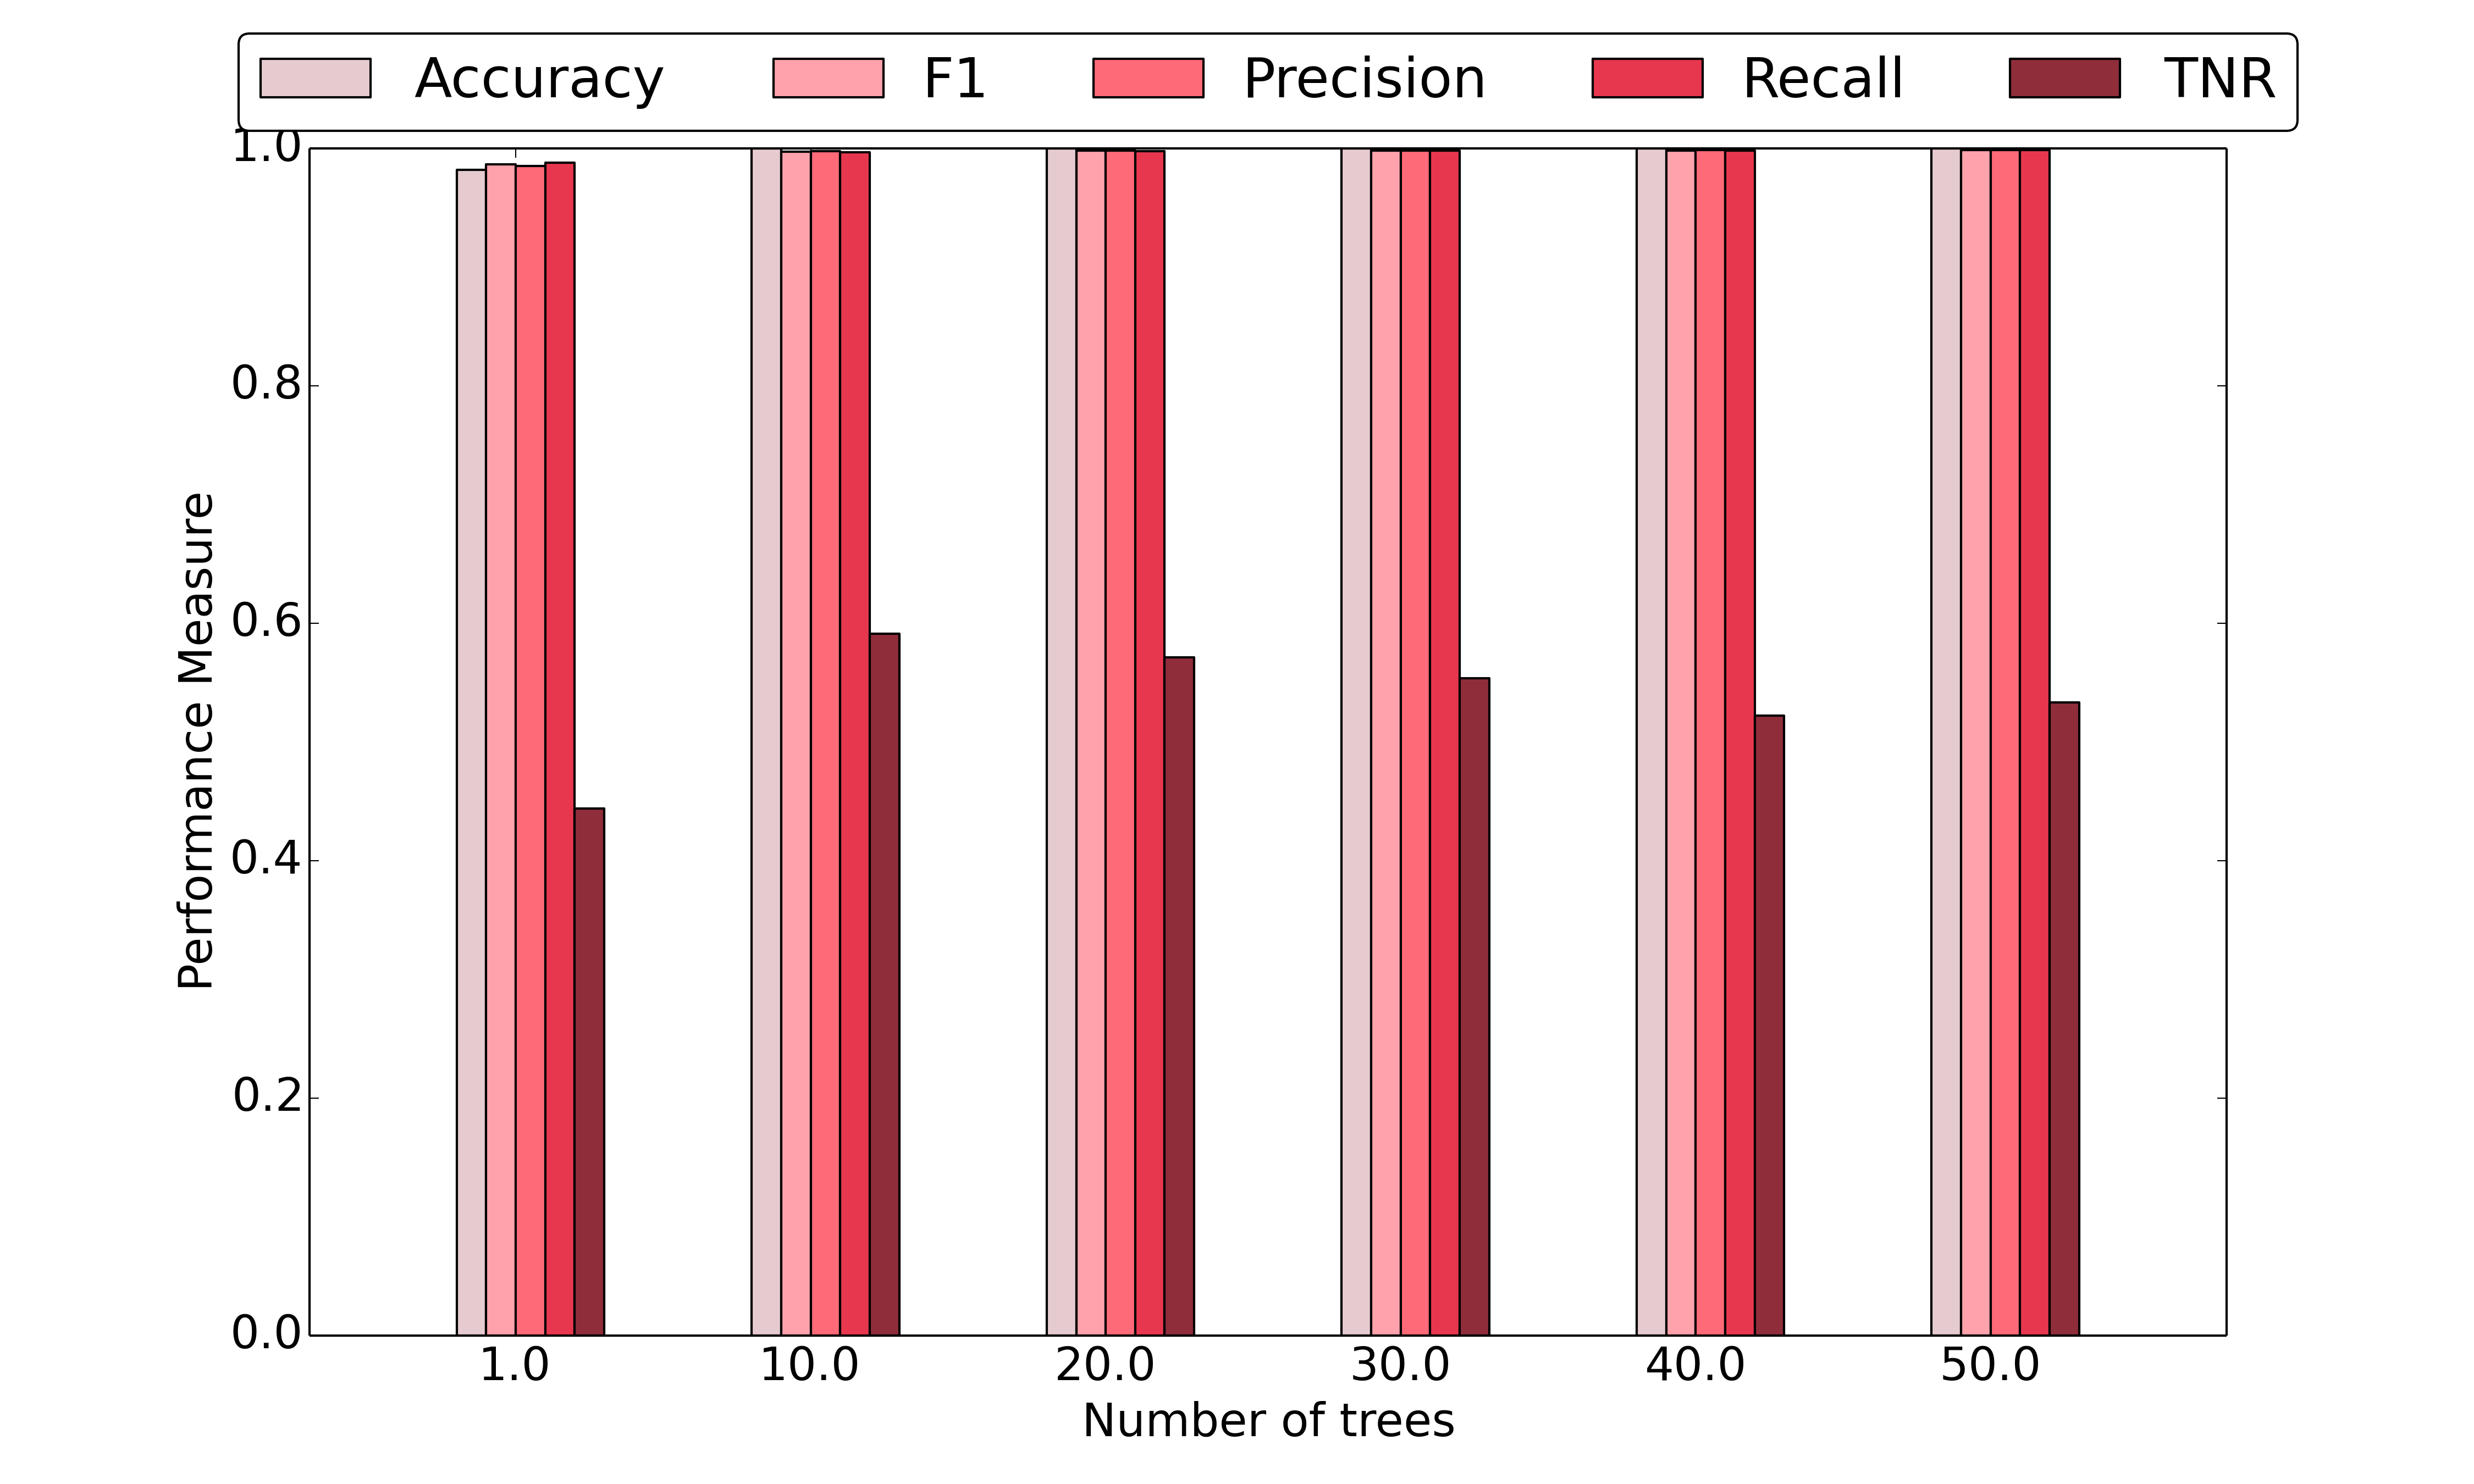
\includegraphics[scale=0.2]{figures/seqPerf.png}
\caption{Sequential code performance with trees in ${1,10,20,30,40}$}
\end{subfigure}
\begin{subfigure}{.4\textwidth}
\centering
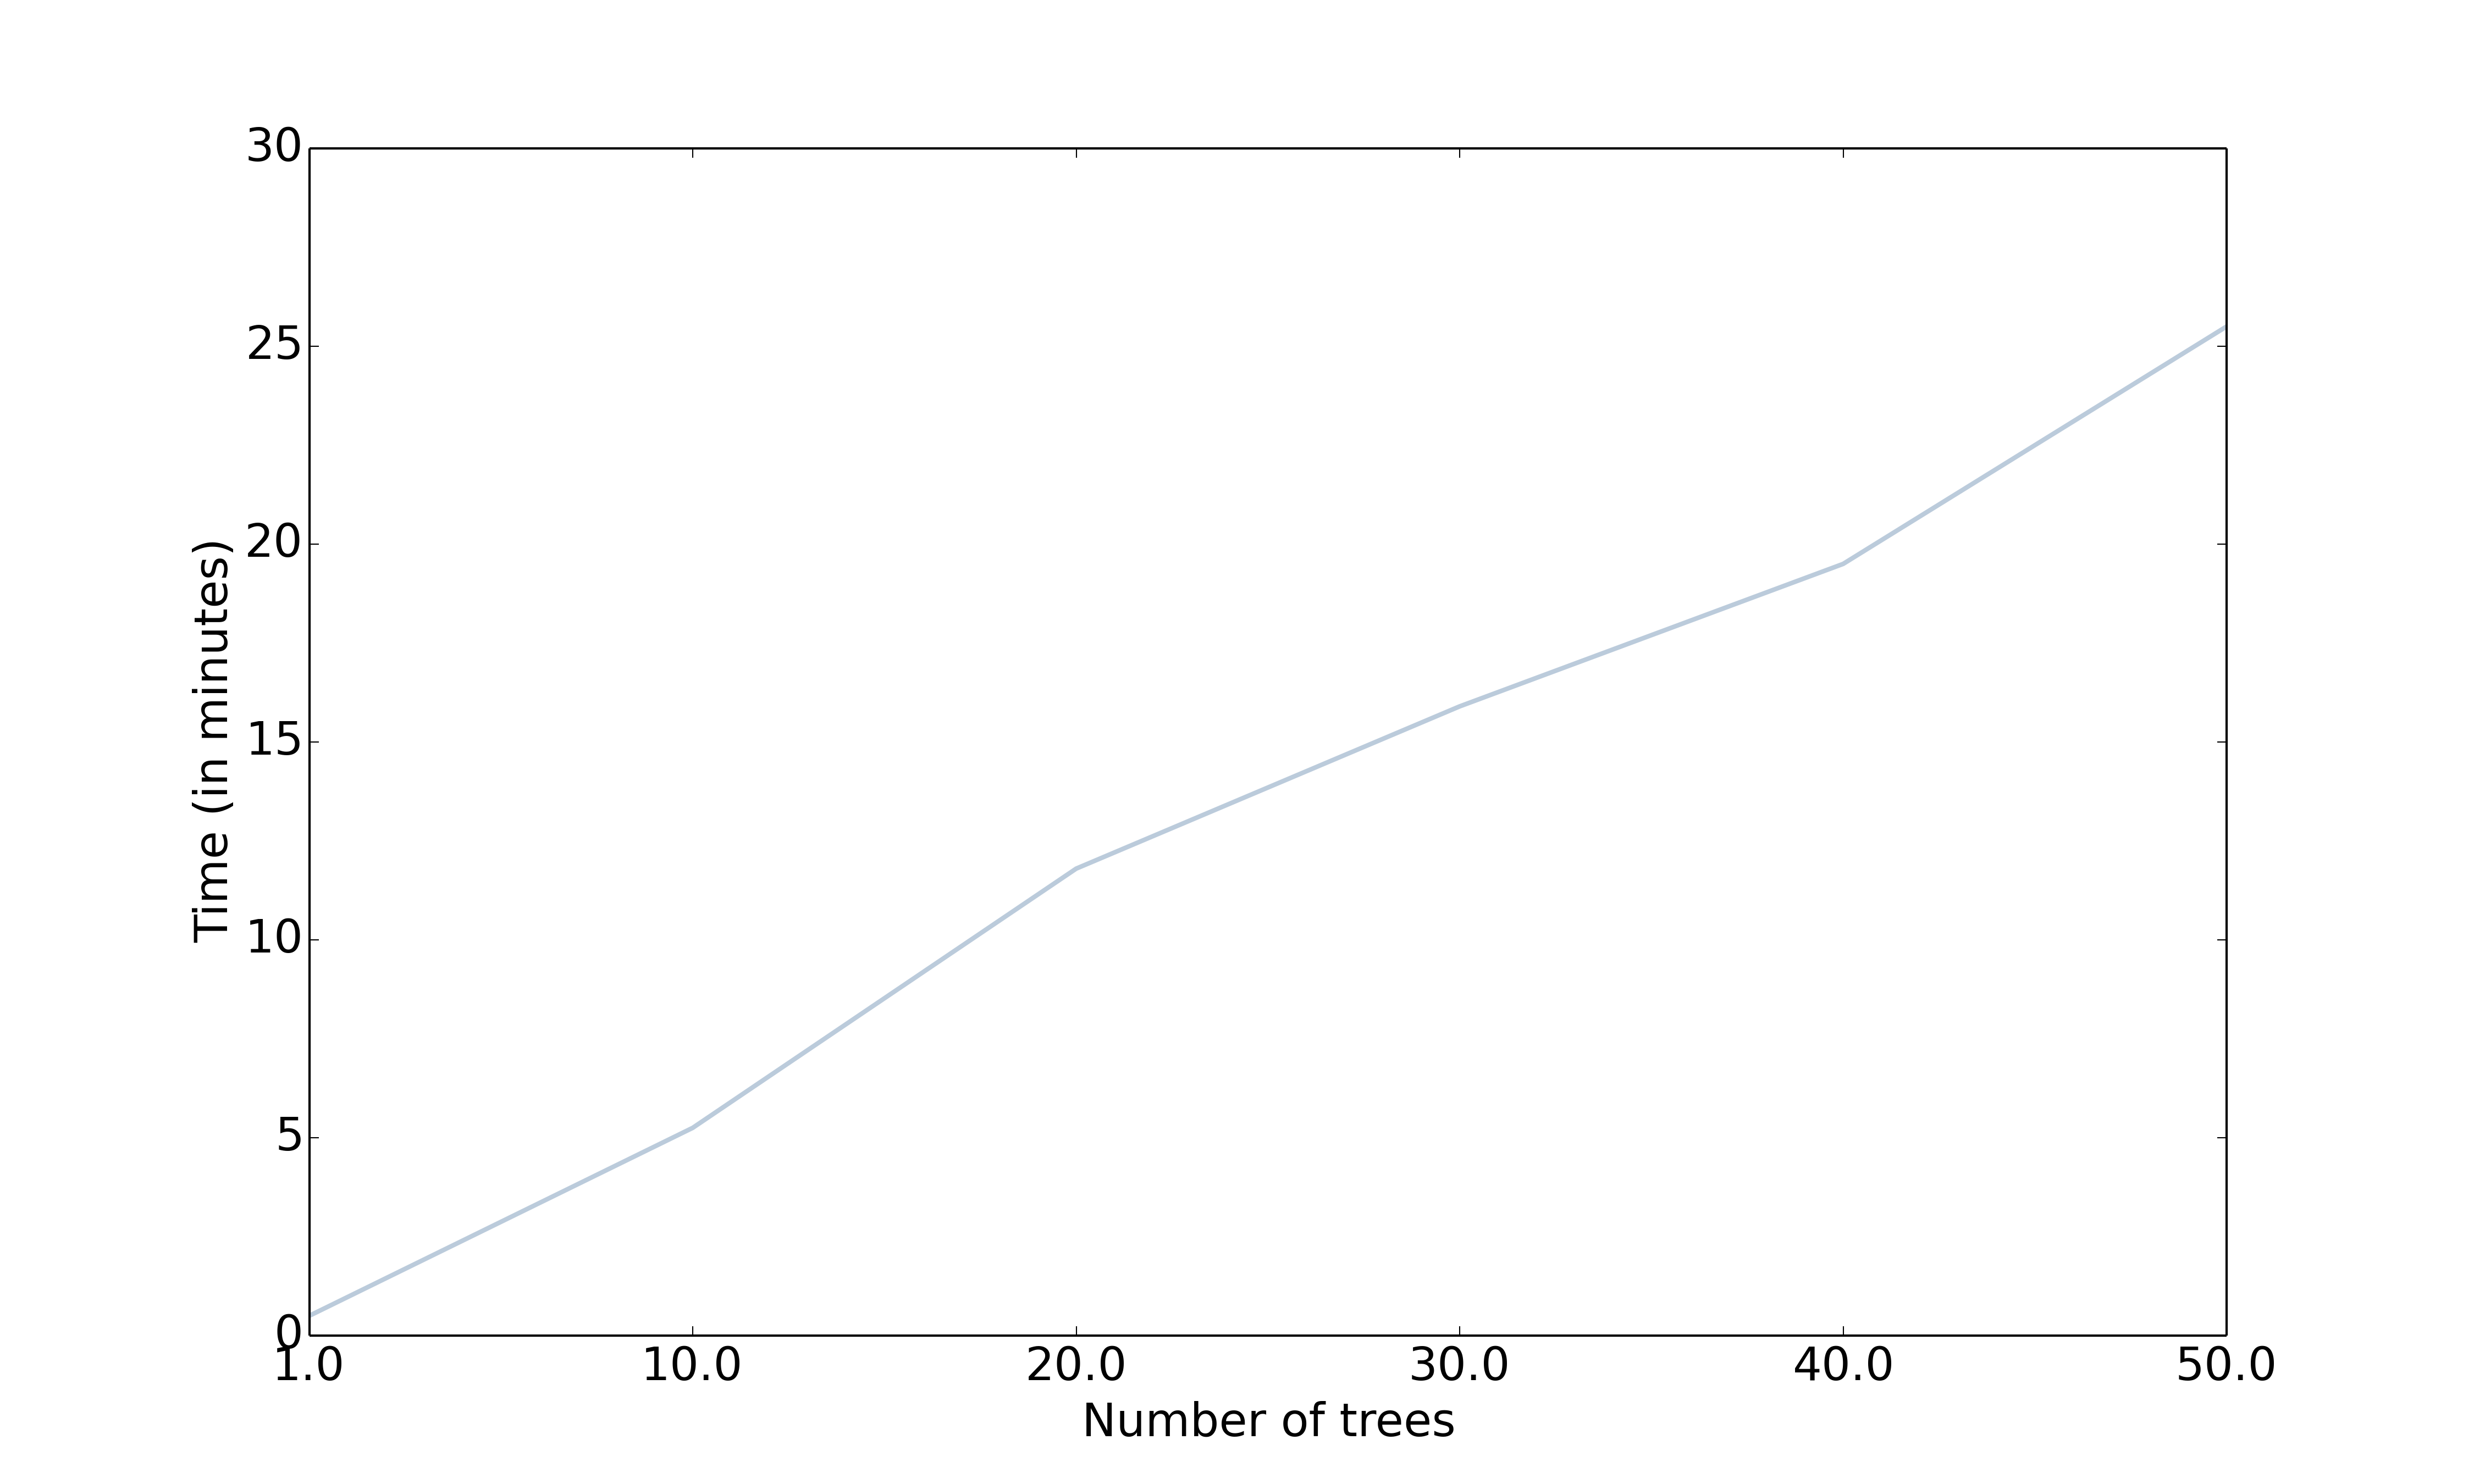
\includegraphics[scale=0.2]{figures/seqTime.png}
\caption{Time taken to construct corresponding trees.}
\end{subfigure}
\caption{Sequential code of Random Forest in \textit{Java ML library}'s performance.}
\label{fig:seqCode}
\end{figure*}

\subsection{Random Forests: Sequential Code}
For our experiments, we utilized both the sequential code provided by \textit{ironmanMA}'s \cite{seqCode} and the sequential code \textit{Java ML} by Thomas Abeel \cite{jmlSeqCode} open source implementation of the Random Forest learning algorithm; initially we worked with \textit{ironmanMA}'s, but then switched to running our experiments with \textit{JavaML}.  We used the \textit{ironmanMA} and \textit{Java ML} open-source implementations of a Random Forest classifier as base, sequential Random Forest models, and then incorporated them into the \textit{Harp} framework.  

We primarily utilized the sequential code provided by \textit{Java ML Library}'s \cite{abeel2009java} open source implementation of the Random Forest algorithm. The \textit{Java ML Library} code is optimized for fast learning of Random forests with continuous and categorical features. We ran some preliminary experiments with \cite{seqCode} sequential code on the \textit{PAMAP2} \cite{reiss2012introducing,reiss2012creating} (described in detail in the Experiments section). In the \textit{PAMAP2} domain, accuracy at the problem task (predicting activities from the dataset) improved as the number of trees in the forest was increased. However, the accuracy difference between 1 tree (22\%) and 50 trees (38\%) is 16\%. 

Given this poor performance of the learning framework for the 18-way classification problem, we simplified the problem to a binary classification task. We do this as we are interested in studying the effect of the different data distributions on the performance of random forests, and the powerful advantage of utilizing a distributed framework for this task. If the Random Forest's performance is deprecated as a result of the distributed environment, it would have been challenging to tell the extent of the deprecation given how poor the performance was for the non-distributed version. Our intended analysis is more beneficial when the models learned have a good performance as a baseline to be compared against; this is achieved by making the task simpler, which emphasizes our focus to the distribution of the data and it's impact on performance. Focusing on the data distribution enabled us to actually compare models. With the task being simplified to a binary task, the sequential code's models have a good performance. Some preliminary results from this experiment are given in Figure !!!. As can be seen, the time taken by the sequential code increases linearly, and therefore we cap the number of trees at 50 in this case. With this \textit{achievable, realistic} performance of the algorithm on this data, we compare various data configurations, their impact on performance, and the pros and cons offered by a distributed parallel framework. 

The performance scores reported for multi-class classification are the result of running the \textit{ironmanMA} sequential Random Forest. This is the only place where results for  \textit{ironmanMA}'s code is reported. We switched to running \textit{Java ML} for our distributed experiments due to the extreme extent to which \textit{ironmanMA}'s implementation was computationally inefficient; both in terms of time and space complexity. The \textit{ironmanMA}'s implementation was so inefficient that we do not believe it to be compatible neither \textit{Harp} not \textit{Hadoop}, nor do we believe it to be compatible with machine learning problems that need to solved at scale. Therefore, all results and experiments in the rest of this paper are reported with respect to the \textit{Java ML} implementation of Random Forest.

\iffalse
The sequential code provided by \textit{ironmanMA}'s \cite{seqCode} open source implementation of the Random Forest learning algorithm. This code utilizes threads to learn the trees that constitute the forest in a parallel fashion, but here we restrict the numThreads setting to be 1, to show the inefficiency of the code in a truly sequential mode. We ran some preliminary experiments with \textit{ironmanMA}'s sequential code on the \textit{PAMAP2} \cite{reiss2012introducing,reiss2012creating} (described in detail in the Experiments section). In \textit{PAMAP2} domain, accuracy of the problem task (predicting activities from the dataset) improved as the number of trees was increased. However, the accuracy difference between 1 tree (22\%) and 50 trees (38\%) is 16\% while the time difference is 43 minutes. This is problematic as it will likely take about 500 trees in the forest before the classifier becomes useful while the required learning time increases at a much father rate than the accuracy does relative to the number of trees. This means that it will likely take about 10 hours to learn a forest of size 500. This is not feasible, especially once it is considered that all results presented here are with respect to training on only $\frac{1}{9}^{th}$ of the overall data set. Results are reported on  $\frac{1}{9}^{th}$ of the overall data set as we were restricted to subsampling the train data from the whole dataset based on the limited computing resources on our personal computers. Additionally, using the entire data set caused “Out of Memory Errors”. The occurence of an "Out of Memroy Error" when trying to load the entire training data set into memory is a strong indication for the need of a distributed implmentation of the Random Forest classifier in order to make predictions in the \textit{PAMAP2} domain. Therefore, any distributed solution needs to account for the size of the data set by distributing the static data as well as distributing the learning process. Table \ref{seqResultsTable} details our experiments with different numbers of trees in the forest and the corresponding accuracy and timing (learn, and test) for 40,316 samples.

\begin{table}[]
\centering
\caption{Sequential code experiments}
\label{seqResultsTable}
\begin{tabular}{|l|l|l|l|}
\hline
\textbf{NumTrees} & \textbf{Accuracy\%} & \textbf{Learn Time} & \textbf{Test time} \\ \hline
1                 & 22                & 1m 13 s             & 1.2 s              \\ \hline
10                & 31                & 8m 59 s             & 2.8 s              \\ \hline
50                & 38                & 42m 39 s            & 13.34 s            \\ \hline
100               & 39                & 1hr 10m             & 24.59 s            \\ \hline
\end{tabular}
\end{table}
\fi

\subsection{Building the training and test data}
Before creating any of the training sets, 20\% of the overall data points across subjects were randomly sampled, withheld, and removed from the data set for use as a test/evaluation set.

For the first set of eight subsets of the \textit{PAMAP2} data, \textit{Local-Feature-Label data}, we combined the last two subject files since the last two subjects had really low number of samples (plus given that we utilized an even number of nodes on Juliet clusters, this configuration is applicable). The combined subject files were used as our training set partitions. As each of the original data subsets was generated by a different person, they should each have a different distribution over the feature values, because each person would have completed the activities in their own way. Additionally, as each participant only completed a subset of the 18 activities, the distribution over the classes also differs between the different subsets. Therefore this organization is representative of differing local feature-label distributions.

For the second set of eight subsets of the \textit{PAMAP2} data,\textit{Local-Label data}, we created the data partitions by randomly sampling across all participants (minus the 20\% of data points that were selected for testing) such that each of the eight partitions had a uniquely specified distribution over the class values. For this we did not require that the eight subsets have a specific (same or different) distribution over the feature values. 

Each of the eight training data subsets, across the two sets described above, was treated as a unique, "geographical location" by spawning a Random Forest mapper and learning a mini-forest for each data subset. To learn a mini-forest a bootstrapped data set was created by randomly sampling with replacement for each tree from the data subset assigned to the \textit{Mapper}. As the \textit{Mappers}' data partitions do not satisfy the IID assumption, the IID assumption of the cumulative forest (forest created by addition of all these mini-forests) is violated. This constitutes the \textit{Local-Label data} and \textit{Local-Feature-Label data} experiments. 

The Random Forests learned on the data partitions described above were compared against a Random Forest learned on IID data partitions, \textit{Global data}. We created IID data partitions by having our primary mapper collect all data points not selected for use in the test set and write new data partitions to the HDFS. Each data participation that was written to the HDFS was randomly sampled without replacement. The reasons for using this sampling approach and the exact sampling approach are described in further detail in the below Method section. The training and testing set used for the IID partitions matches those used to create the non-IID eight data partitions described above.

In addition, we experiment with \textit{2 Mappers} and \textit{8 Mappers} for all the forms of data to compare \textit{Approximate Global Models} to \textit{Truly Global Models}.

\section{Method}
Our implementation takes advantage of the available sequential code in tandem with the more robust theoretical guarantees provided by certain adaptations of Random Forest. Since we are working in the framework of \textit{Harp}, the main level of parallelism we exploit is by spawning more \textit{Mappers}, where each \textit{Mapper} corresponds to a geographical region. In our implementation we have distributed the sequential code by distributing the tree learning process such that each Mapper learns a mini-forest. \textit{Java ML library}'s sequential code is used to learn each mini-forest. Each mapper builds a local, mini-forest of some specified size (i.e. 50, 100 or 200). Each mini-forest is built sequentially. We chose to build each mini-forest sequentially due to space limitations. We needed to reduce the number of copies of each data point that existed within a \textit{Mapper} at any given point in time in order to be able to run our desired experiments. In order to  evaluate the effect of variations in the feature and label distributions used to learn each mini-forest, we needed to have at least eight mappers running. Therefore, eight different bootstrapped data bags are bootstrapped in parallel for right different trees that are then learned in parallel. Of course, this is for the \textit{Truly Global models}. Correspondingly, for the \textit{Approximate Global models}, we utilize only 2 mappers (and only 2 sets of the data for Local-data experiments). 

\begin{figure*}[t]
\centering
\begin{subfigure}{.4\textwidth}
\centering
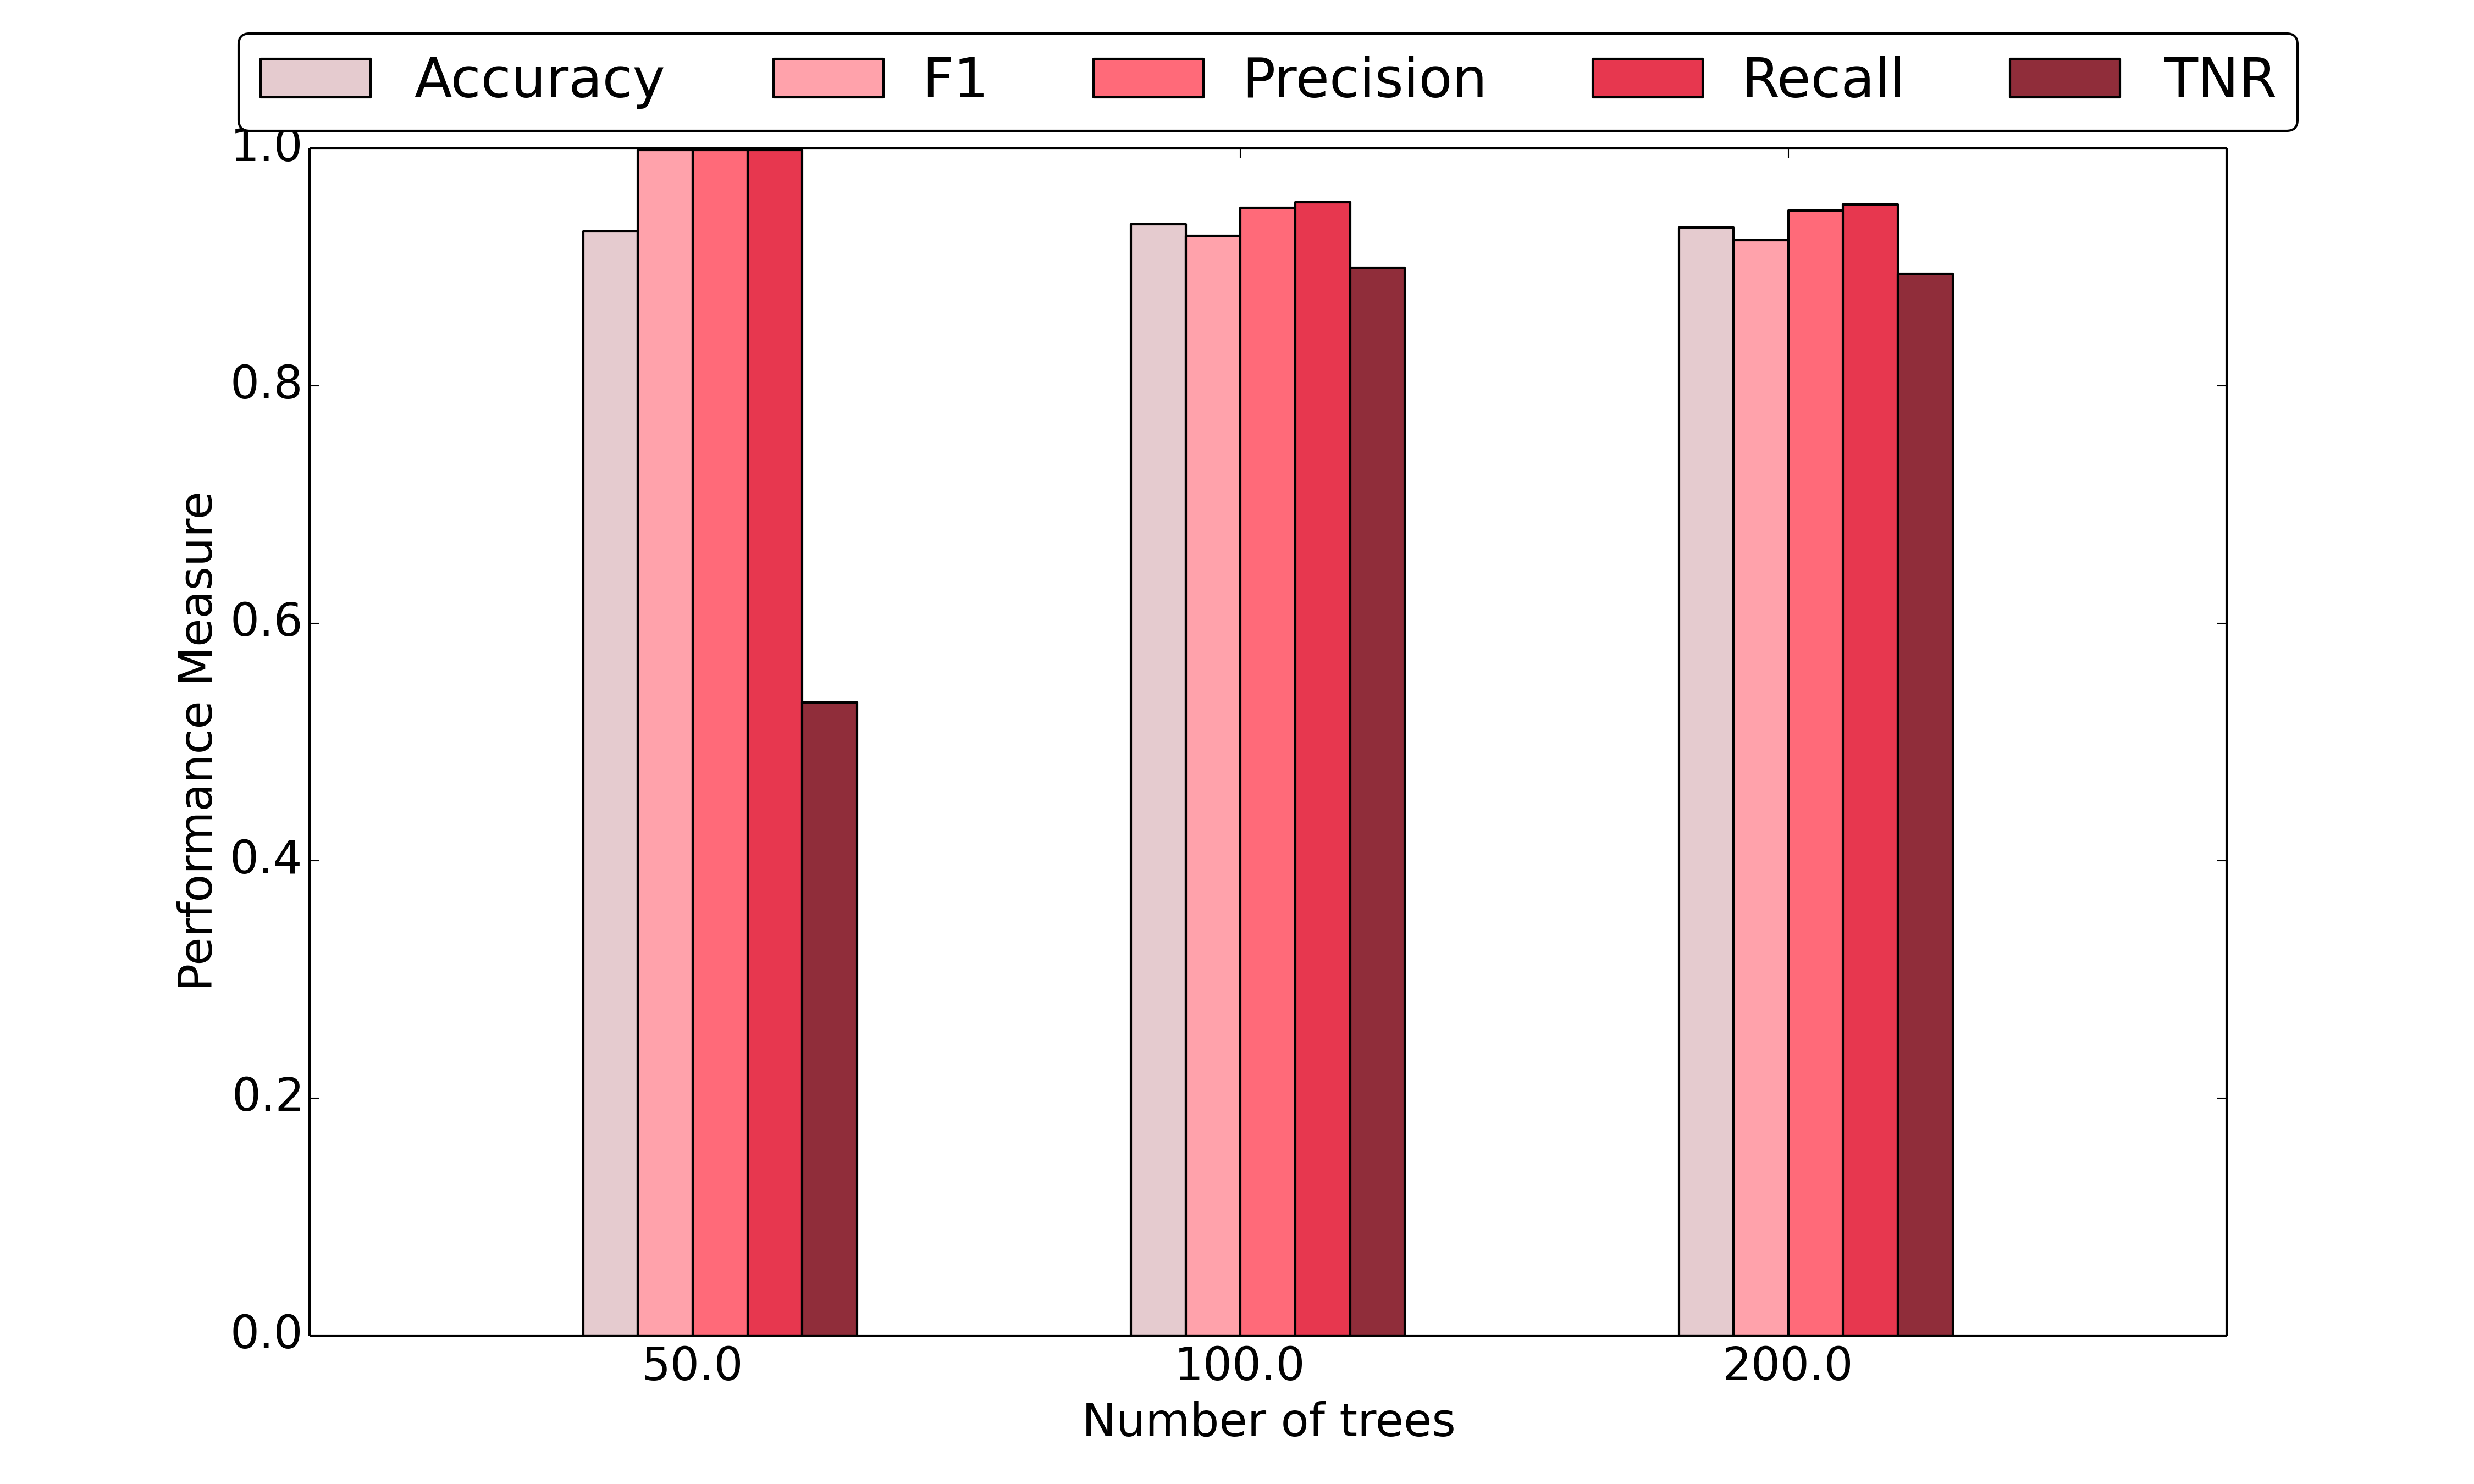
\includegraphics[scale=0.2]{figures/2Map-globalPerf.png}
\caption{\textit{Global data} performance with trees in ${50,100,200}$.}
\end{subfigure}
\begin{subfigure}{.4\textwidth}
\centering
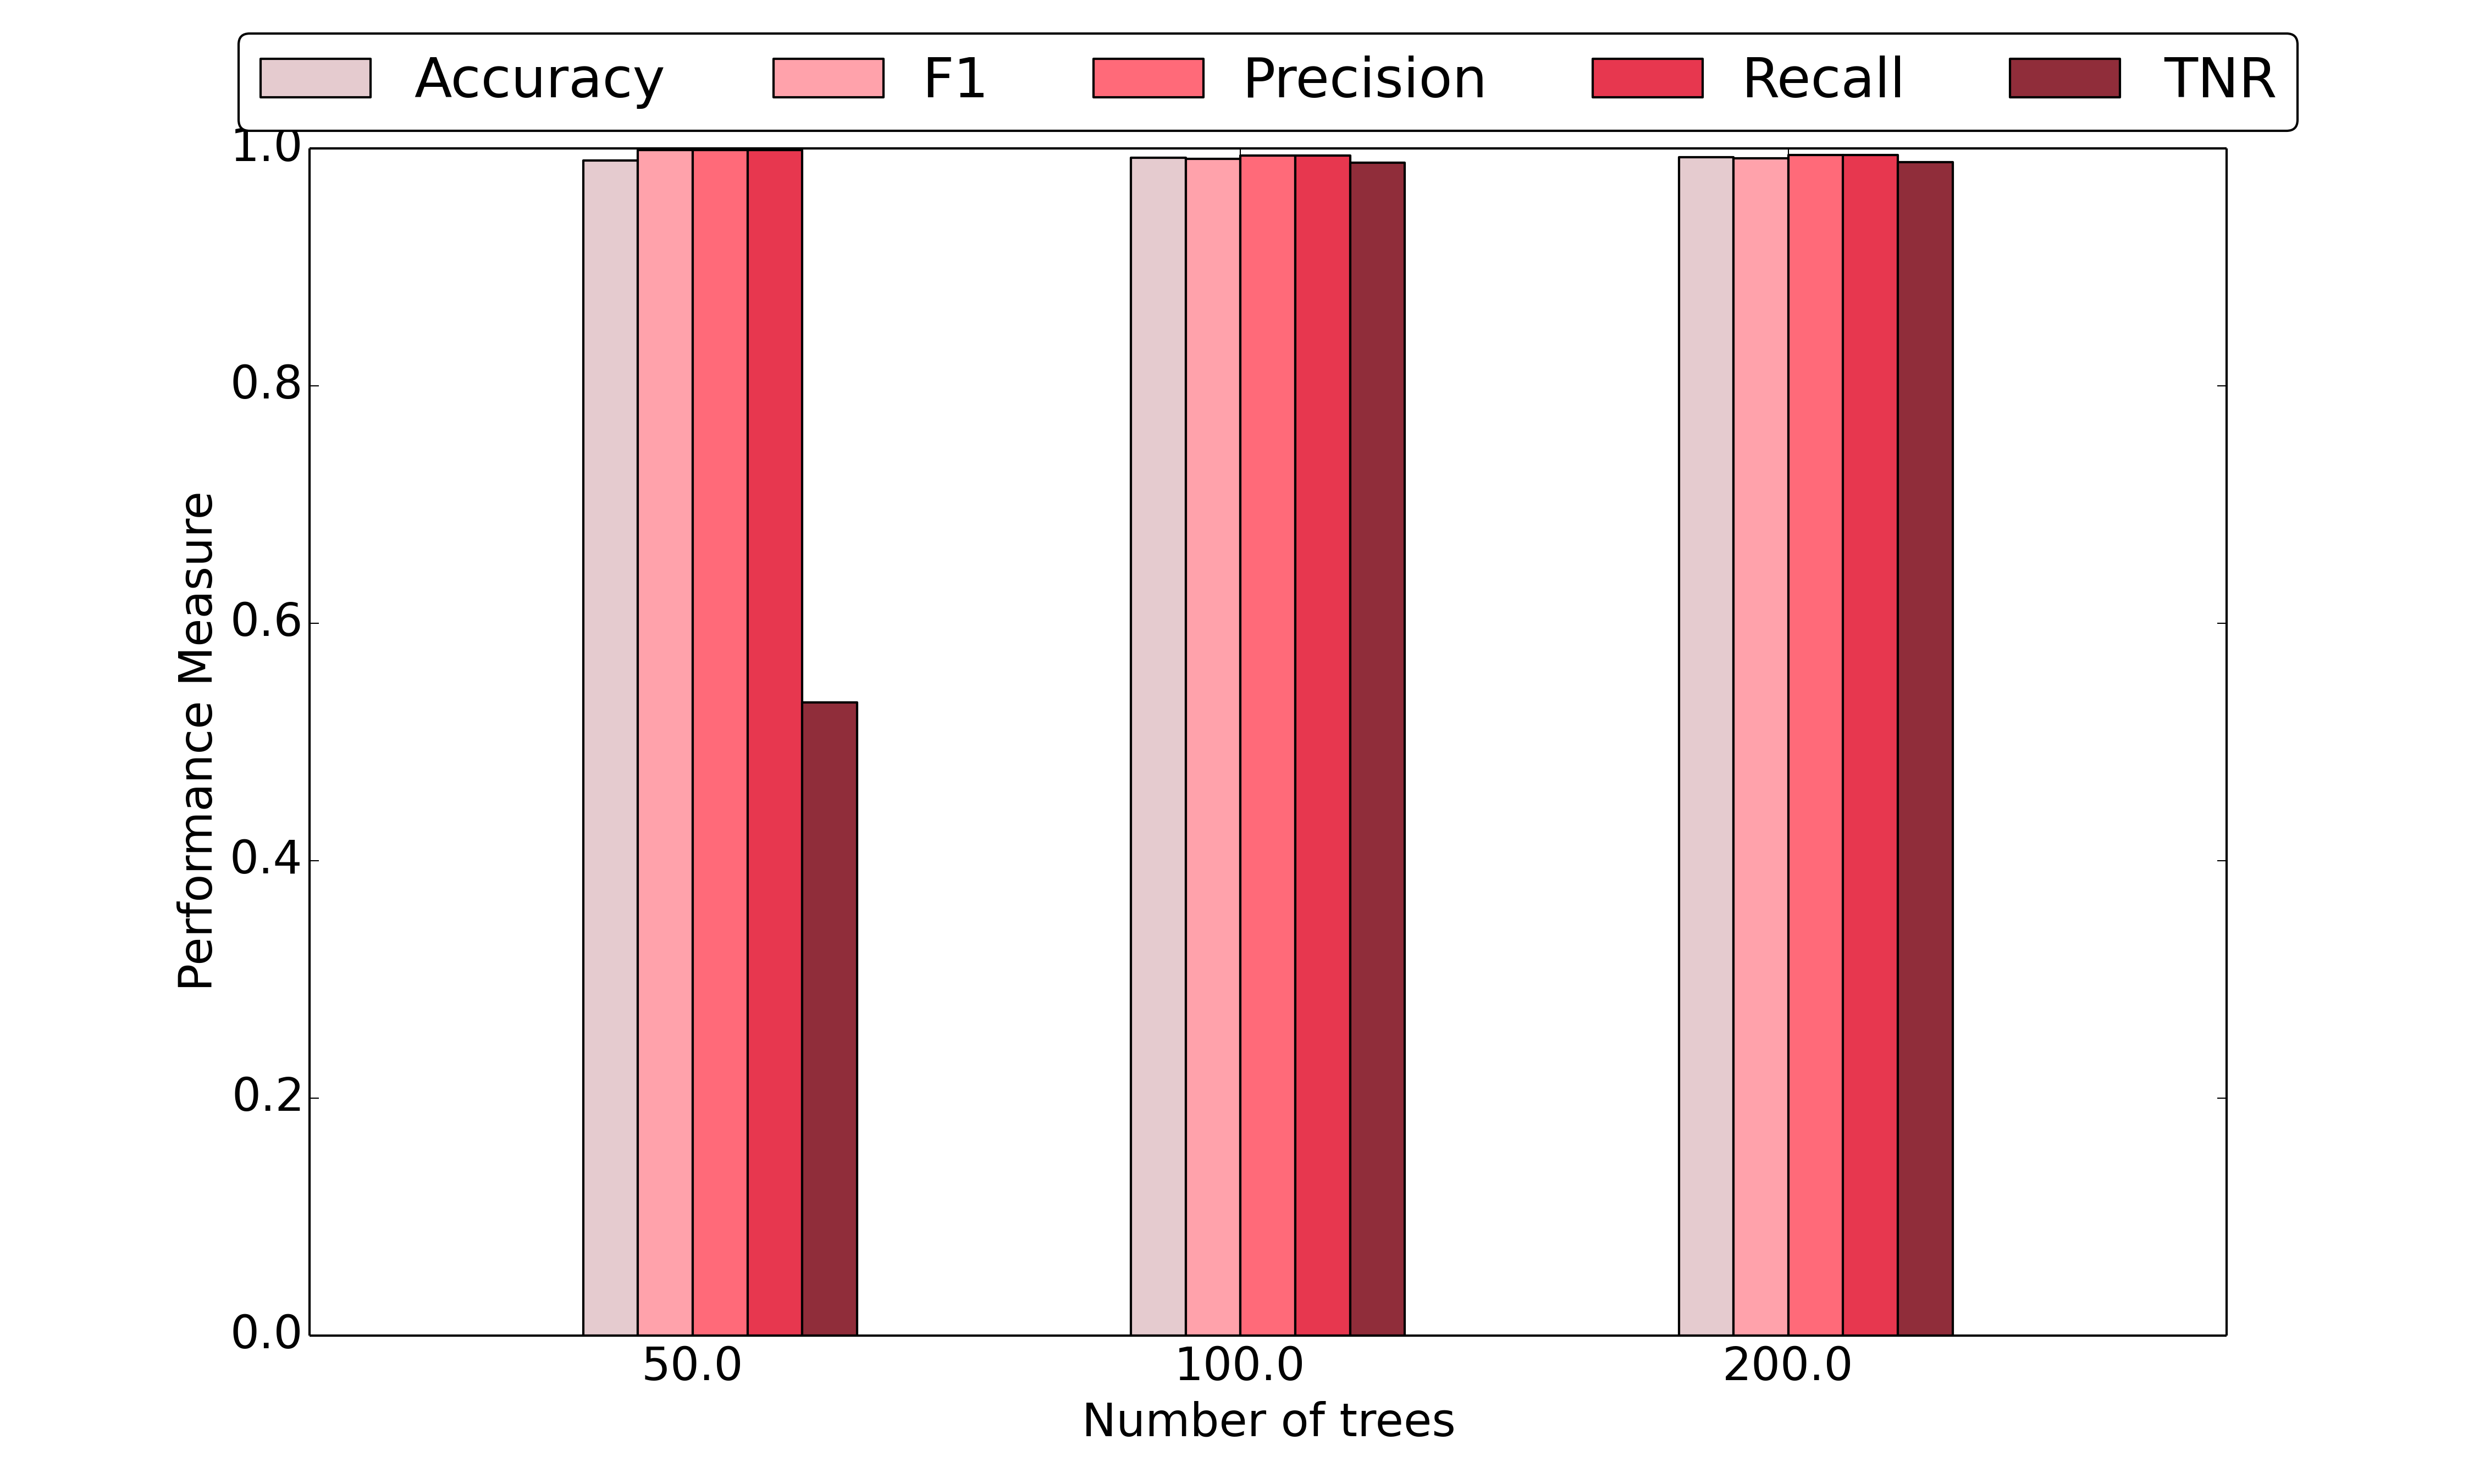
\includegraphics[scale=0.2]{figures/2Map-localLabelPerf.png}
\caption{\textit{Local-Label data} performance with trees in ${50,100,200}$.}
\end{subfigure}
\begin{subfigure}{.4\textwidth}
\centering
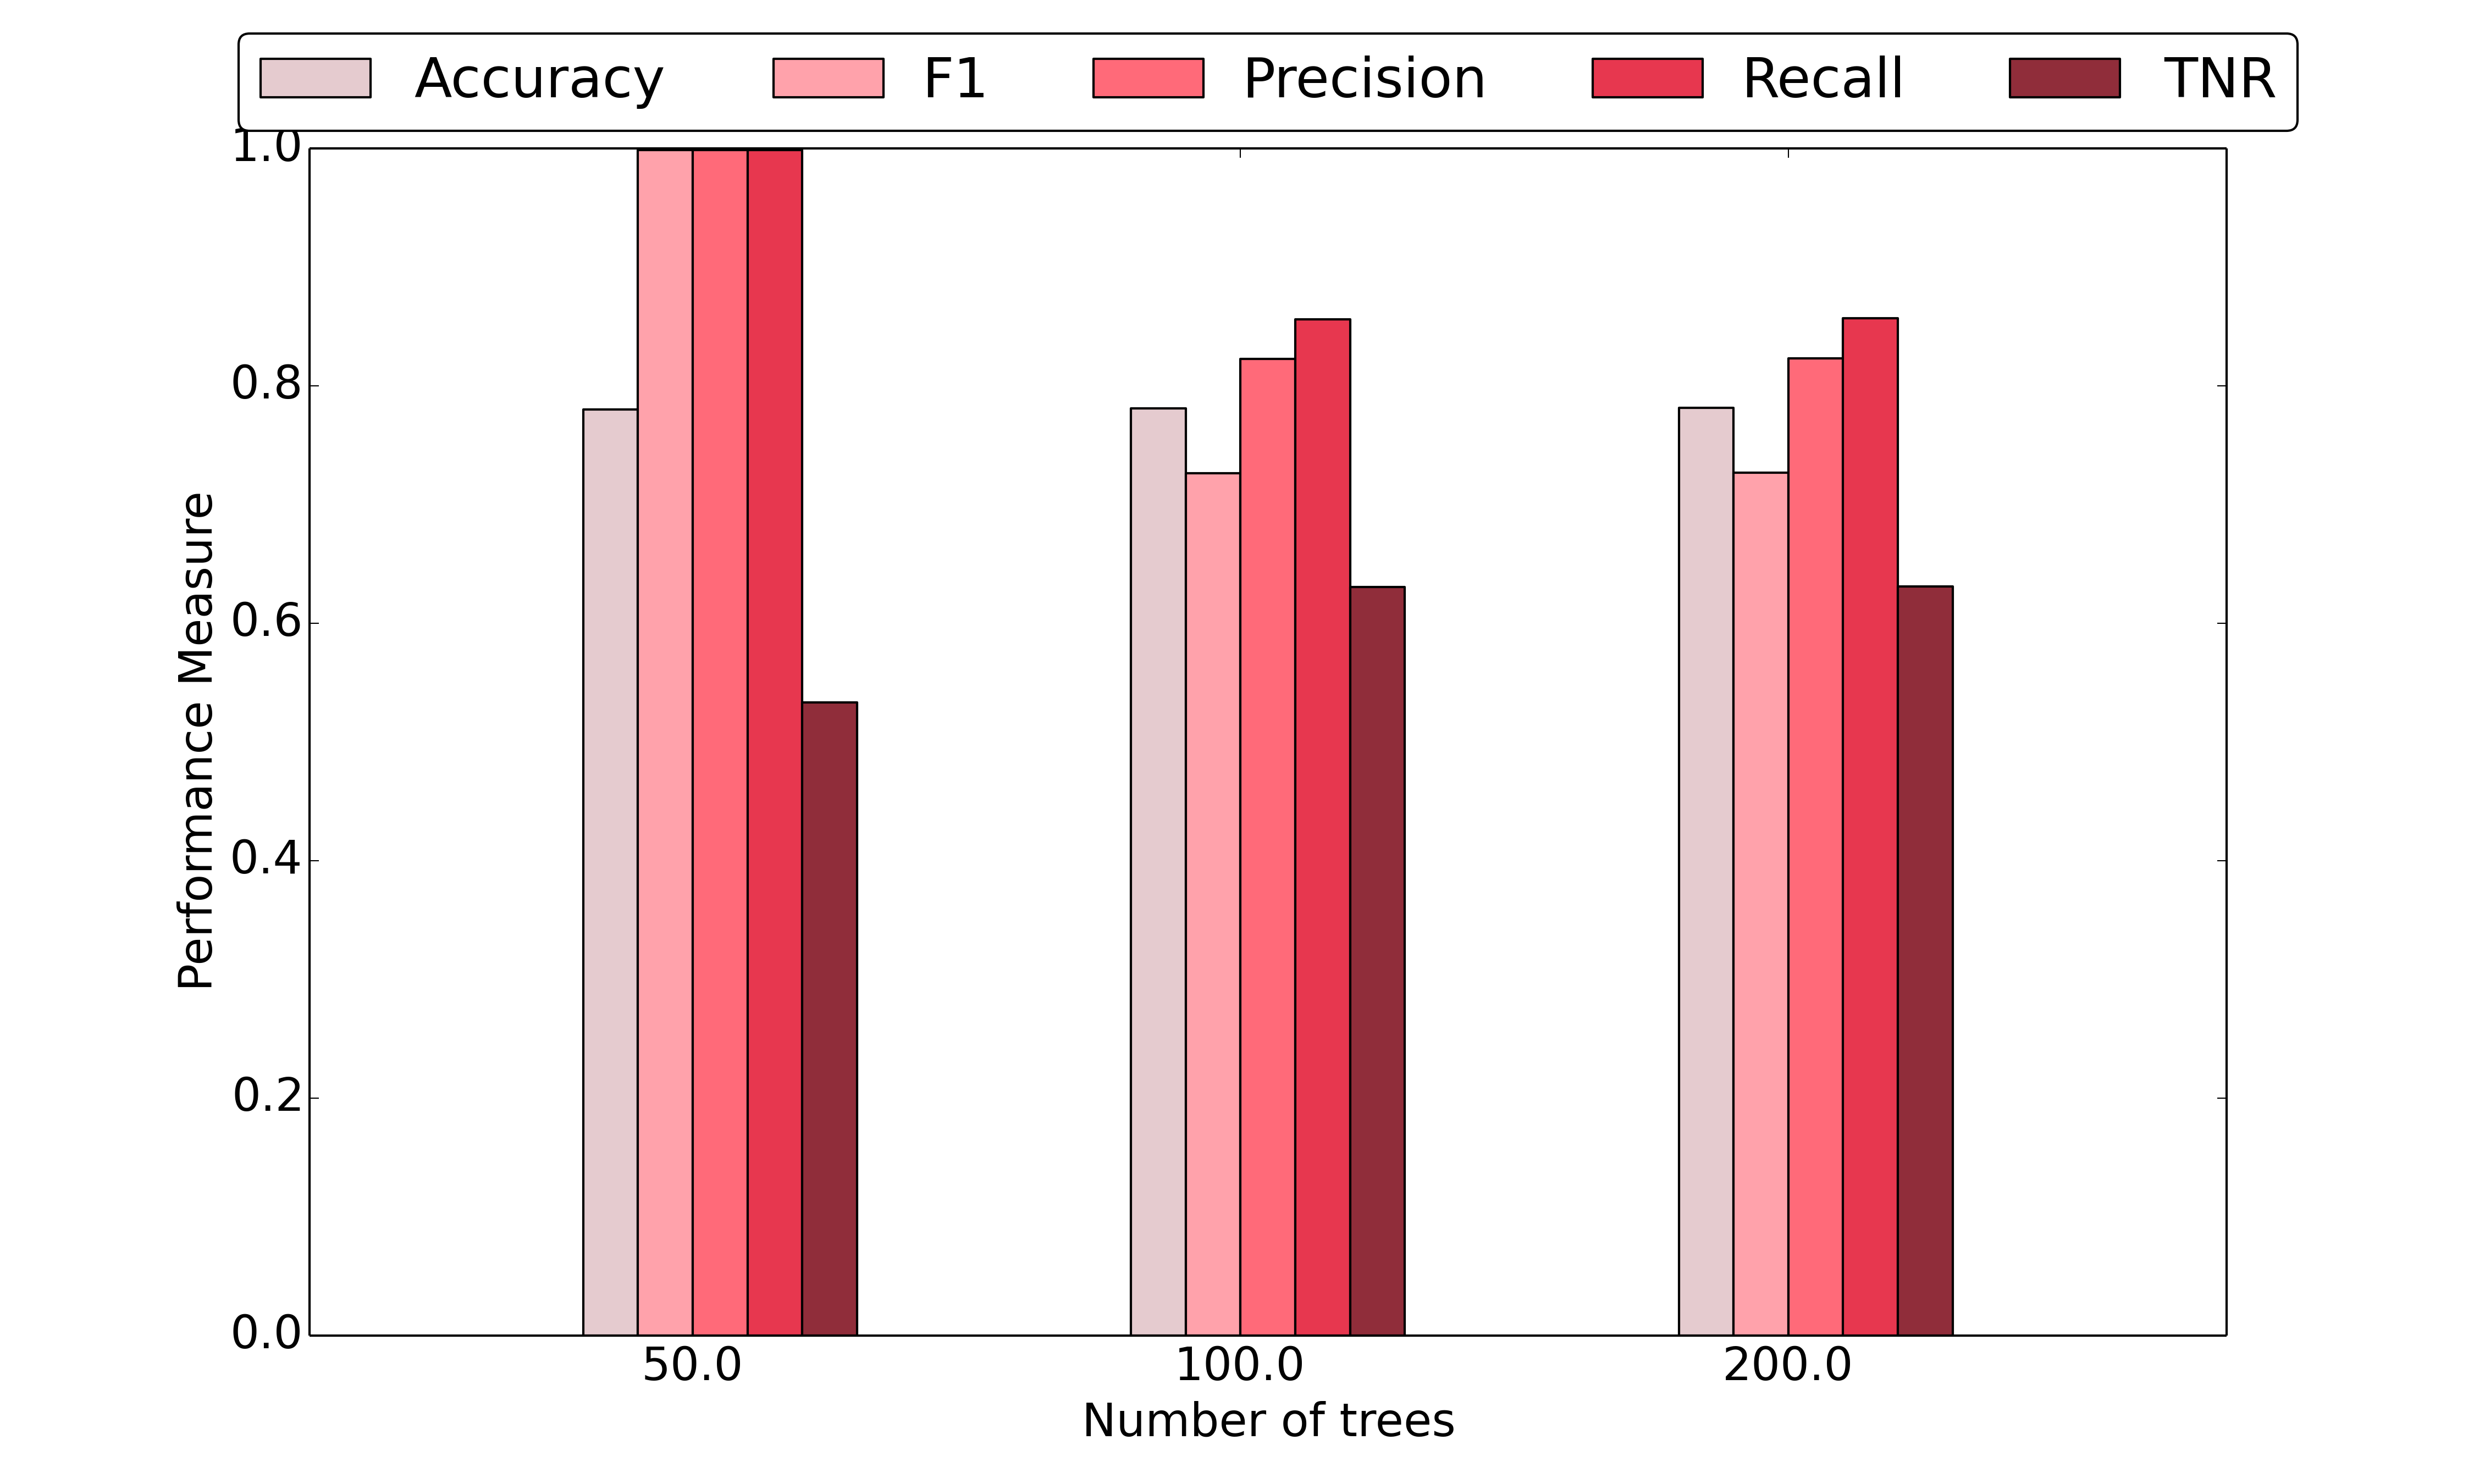
\includegraphics[scale=0.2]{figures/2Map-localFeatureLabelPerf.png}
\caption{\textit{Local-Feature-Label data} performance with trees in ${50,100,200}$.}
\end{subfigure}
\begin{subfigure}{.4\textwidth}
\centering
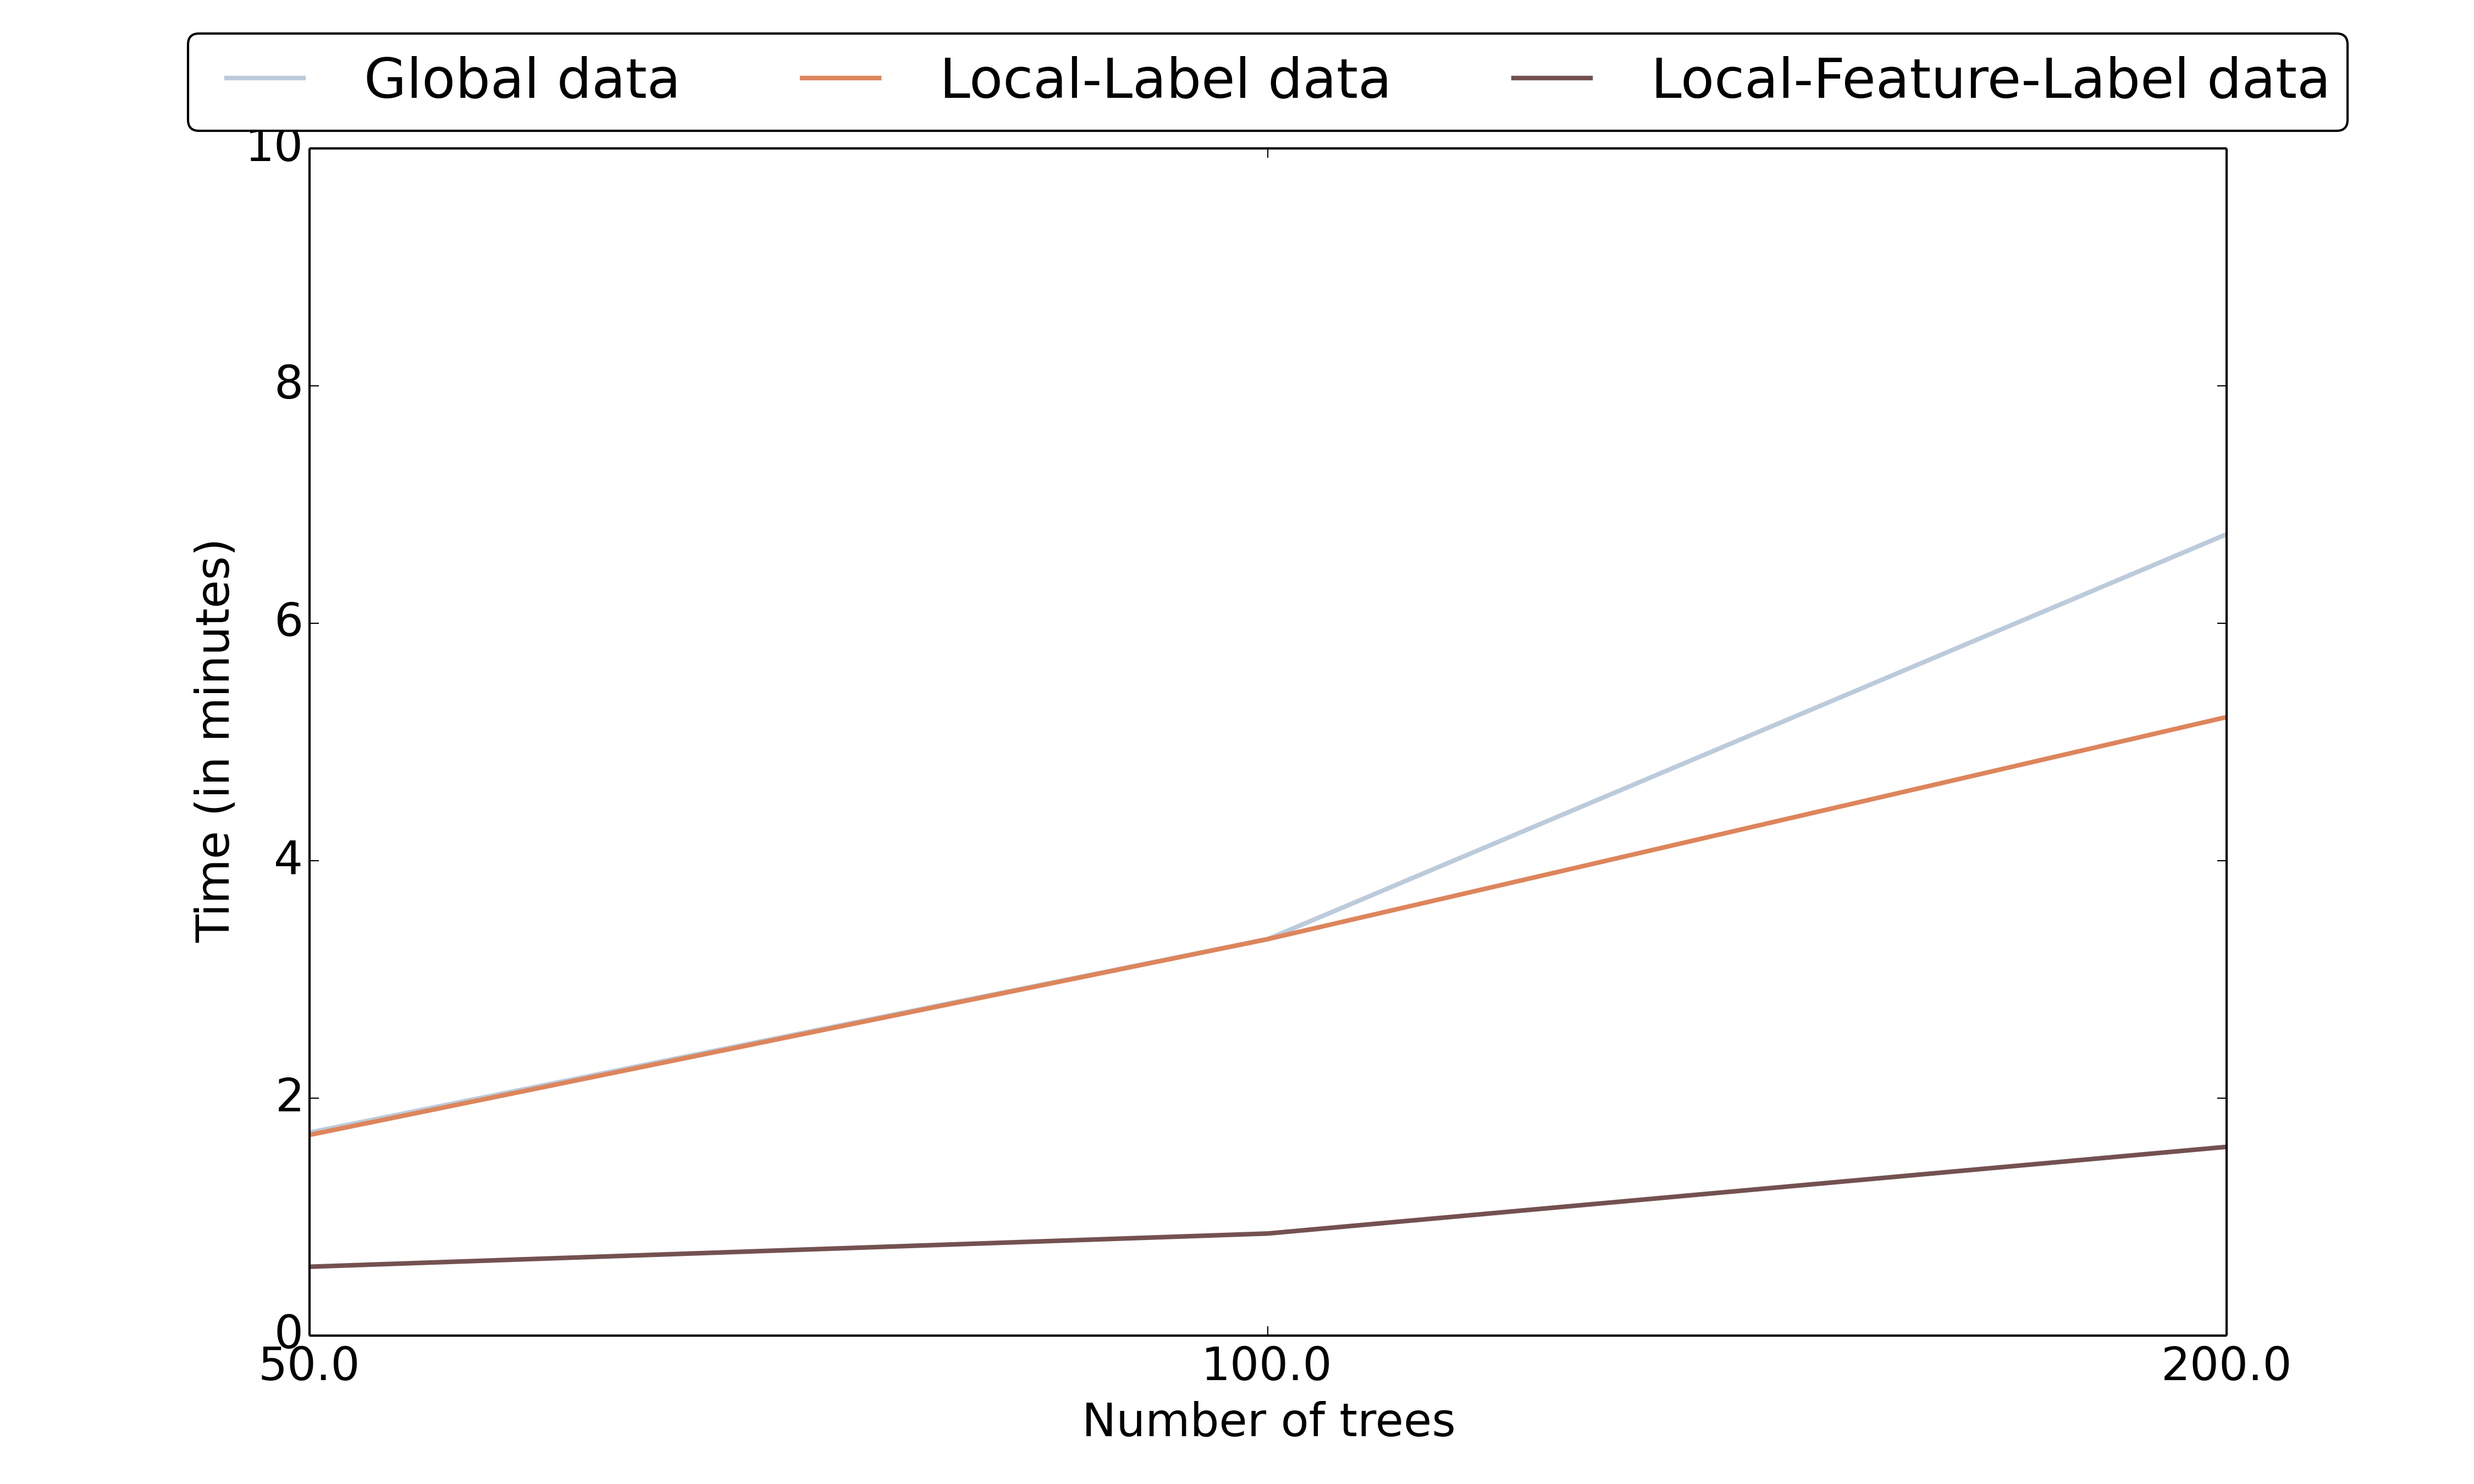
\includegraphics[scale=0.2]{figures/2MapperTime.png}
\caption{Time taken to construct corresponding trees in all corresponding experiments.}
\end{subfigure}
\caption{\textit{Harp}-based parallel code's performance with 2 mappers - \textit{Approximate Global models}.}
\label{fig:approximateGlobalModels}
\end{figure*}


%In our experiments described below, we take and evaluate two different approaches to assigning the data points that will be used to build each of the mini-forests. In the first approach, we assume that each mini-forest is learned from data that was collected from a population with some unique distribution over its feature values and its labels; in the second approach, we assume that each mini-forest is learned from data that represents the global population feature and label distributions. 

In the \textit{Global data} experiments, to control for biases in the distributions over the training data that is used to learn a given mini-forest, we use \textit{Strategic bag-of-little bootstraps} sampling approach. This is essentially bootstrapping without replacement for each tree's dataset. Based on our readings, we have observed that the most robust version of the Random Forest algorithm is the one where each data partition assigned to a given \textit{Mapper} is bootstrapped by sampling without replacement from the global representation of the training data and is used to train one mini-forest. The global forest then consists of all of the trees learned from the different bootstrapped data partitions. Hence, in our case, each \textit{Mapper} learns a mini-forest with respect to a partition of the overall, global data representation, where each mini-forest's trees are trained by sampling with replacement from its local data partitition.

In the \textit{Local data} experiments, we do not try to control for any biases.  Like the \textit{Global data} experiment's mini-forest, the trees in these mini-forests are learned by bootstrapping with replacement. The combination of trees from the multiple \textit{Mappers} forms the global model.
\textit{Strategic bag-of-little bootstraps}.

The predictions from a given mini-forests are combined with those from the mini-forest of all other Mappers to create our global model; our distributed process bootstraps data for and learns 8 (or 2) different trees in parallel where each of the 8 (or 2) trees belong to a different mini-forest. We do not create a global forest that contains all of the learned trees from each of the mini-forests, because the space complexity of this combined model may be huge, and this is not a model we weish to reuse in the perspective of this project. Instead, we collect each mini-forest's predictions on the global test data set to create a global "model" of the test data points being evaluated. In order to distribute the prediction task we can distribute the data and/or we can distribute the model. We have chosen to distribute the model when doing predictions rather than the data. Again, our decision was in a large part motivated by the amount of space that would be required to store the entire forest within each Mapper/task. Therefore, instead of building a global model of the forest, we pass around the test data's feature vectors and the mini-forests' predictions. The predictions from each of the mini-forests are collected, where a mini-forest's predictions consists of a tally of the number of trees that "voted" for each possible class label. The data points are assigned their global class based on the mode of this distribution. The inter-node computation model we are using within \textit{Harp} is model \textit{B} via \textit{AllReduce()}. 
%In the figure below the psuedocode describing how we leverage \textit{Harp} can be seen below:

\subsection{Evaluation}
After the Random Forests for each of the types of distributions on the data partitions described above was learned, they were evaluated on the designated test set. The performance of the models are measured by the following standard statistics: (1) accuracy , (2) F1 score, (3) Precision, (4) Recall, and (5) True negative rate (TNR). We also measure time to quantify the gain offered by utilizing parallel processing. 

\textbf{Sequential experiments:} As a baseline, we record the performance of the sequential code \textit{Java ML library}. These experiments are done on a single dataset of 50 thousand train samples (the test set is the same as those used in the parallel experiments). It must be noted that with a million train samples, the algorithm was unable to learn a single tree even after an hour. So we do not experiment with more samples in the sequential code. These results are given in the Figure \ref{fig:seqCode}. The linear increase in computational time with the increase in the number of trees can be seen prominently, and therefore we explore reducing this computational overhead by parallelizing this framework. 

\begin{figure*}[t]
\centering
\begin{subfigure}{.4\textwidth}
\centering
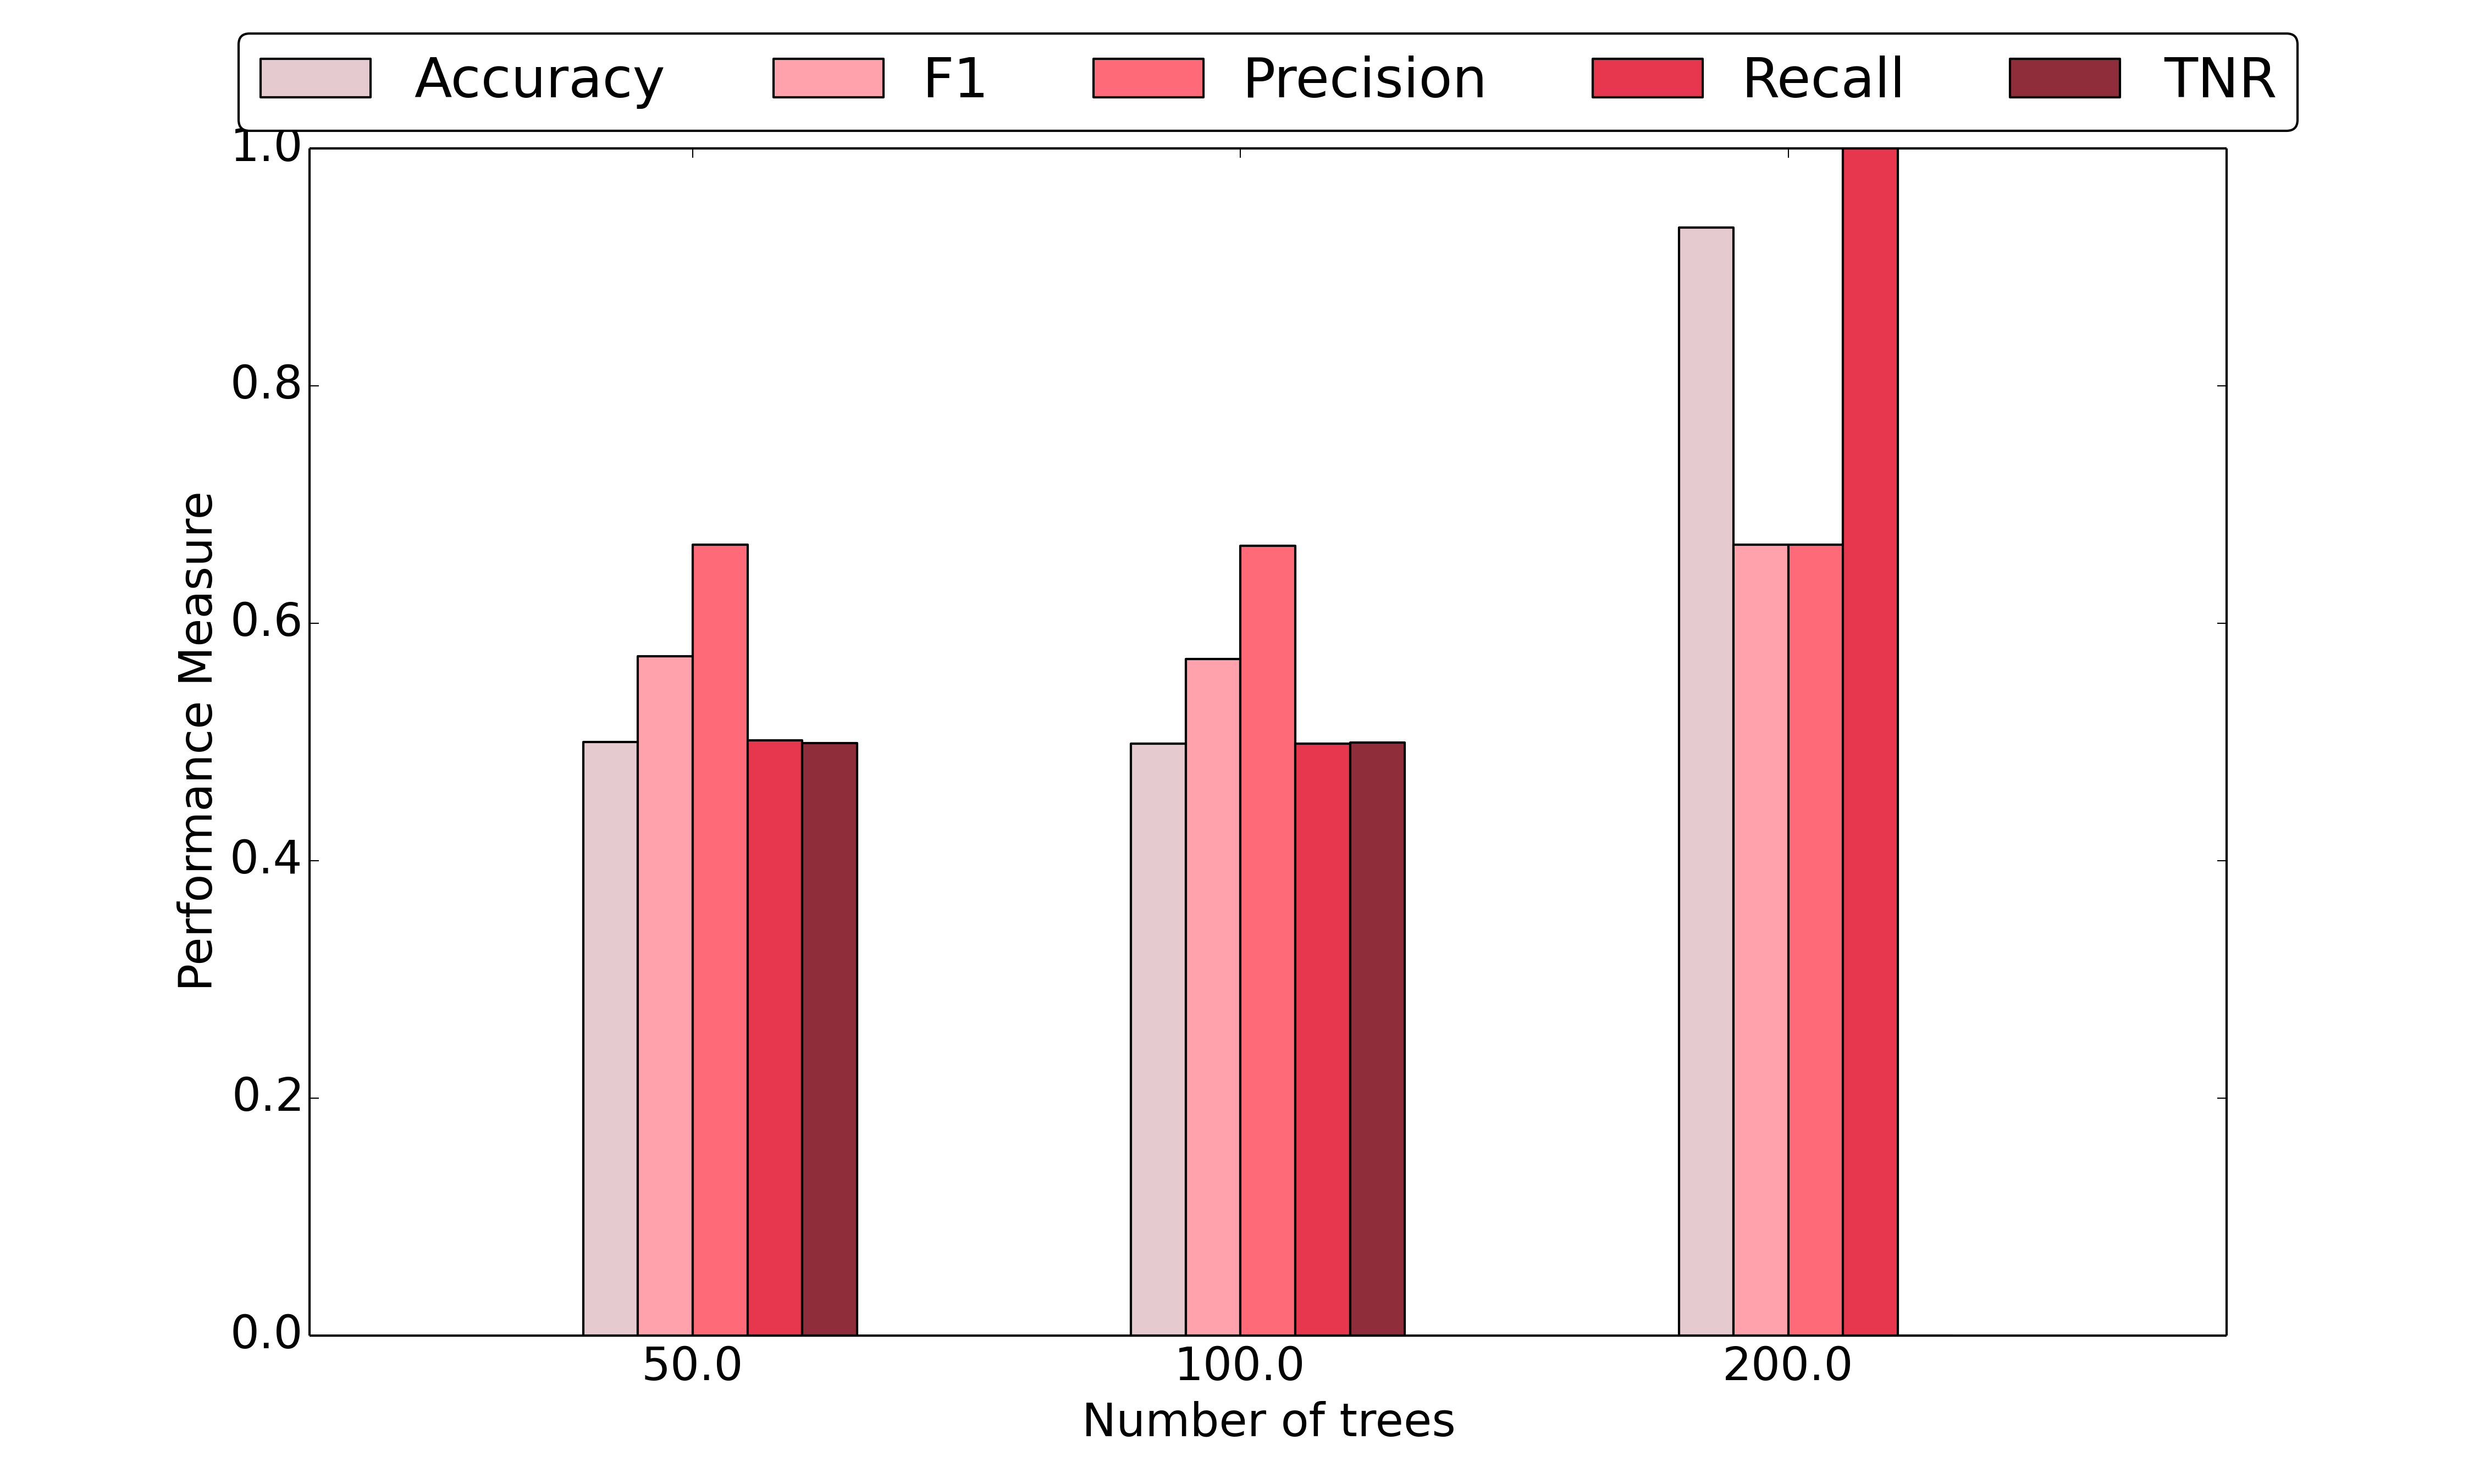
\includegraphics[scale=0.2]{figures/8Map-globalPerf.png}
\caption{\textit{Global data} performance with trees in ${50,100,200}$.}
\end{subfigure}
\begin{subfigure}{.4\textwidth}
\centering
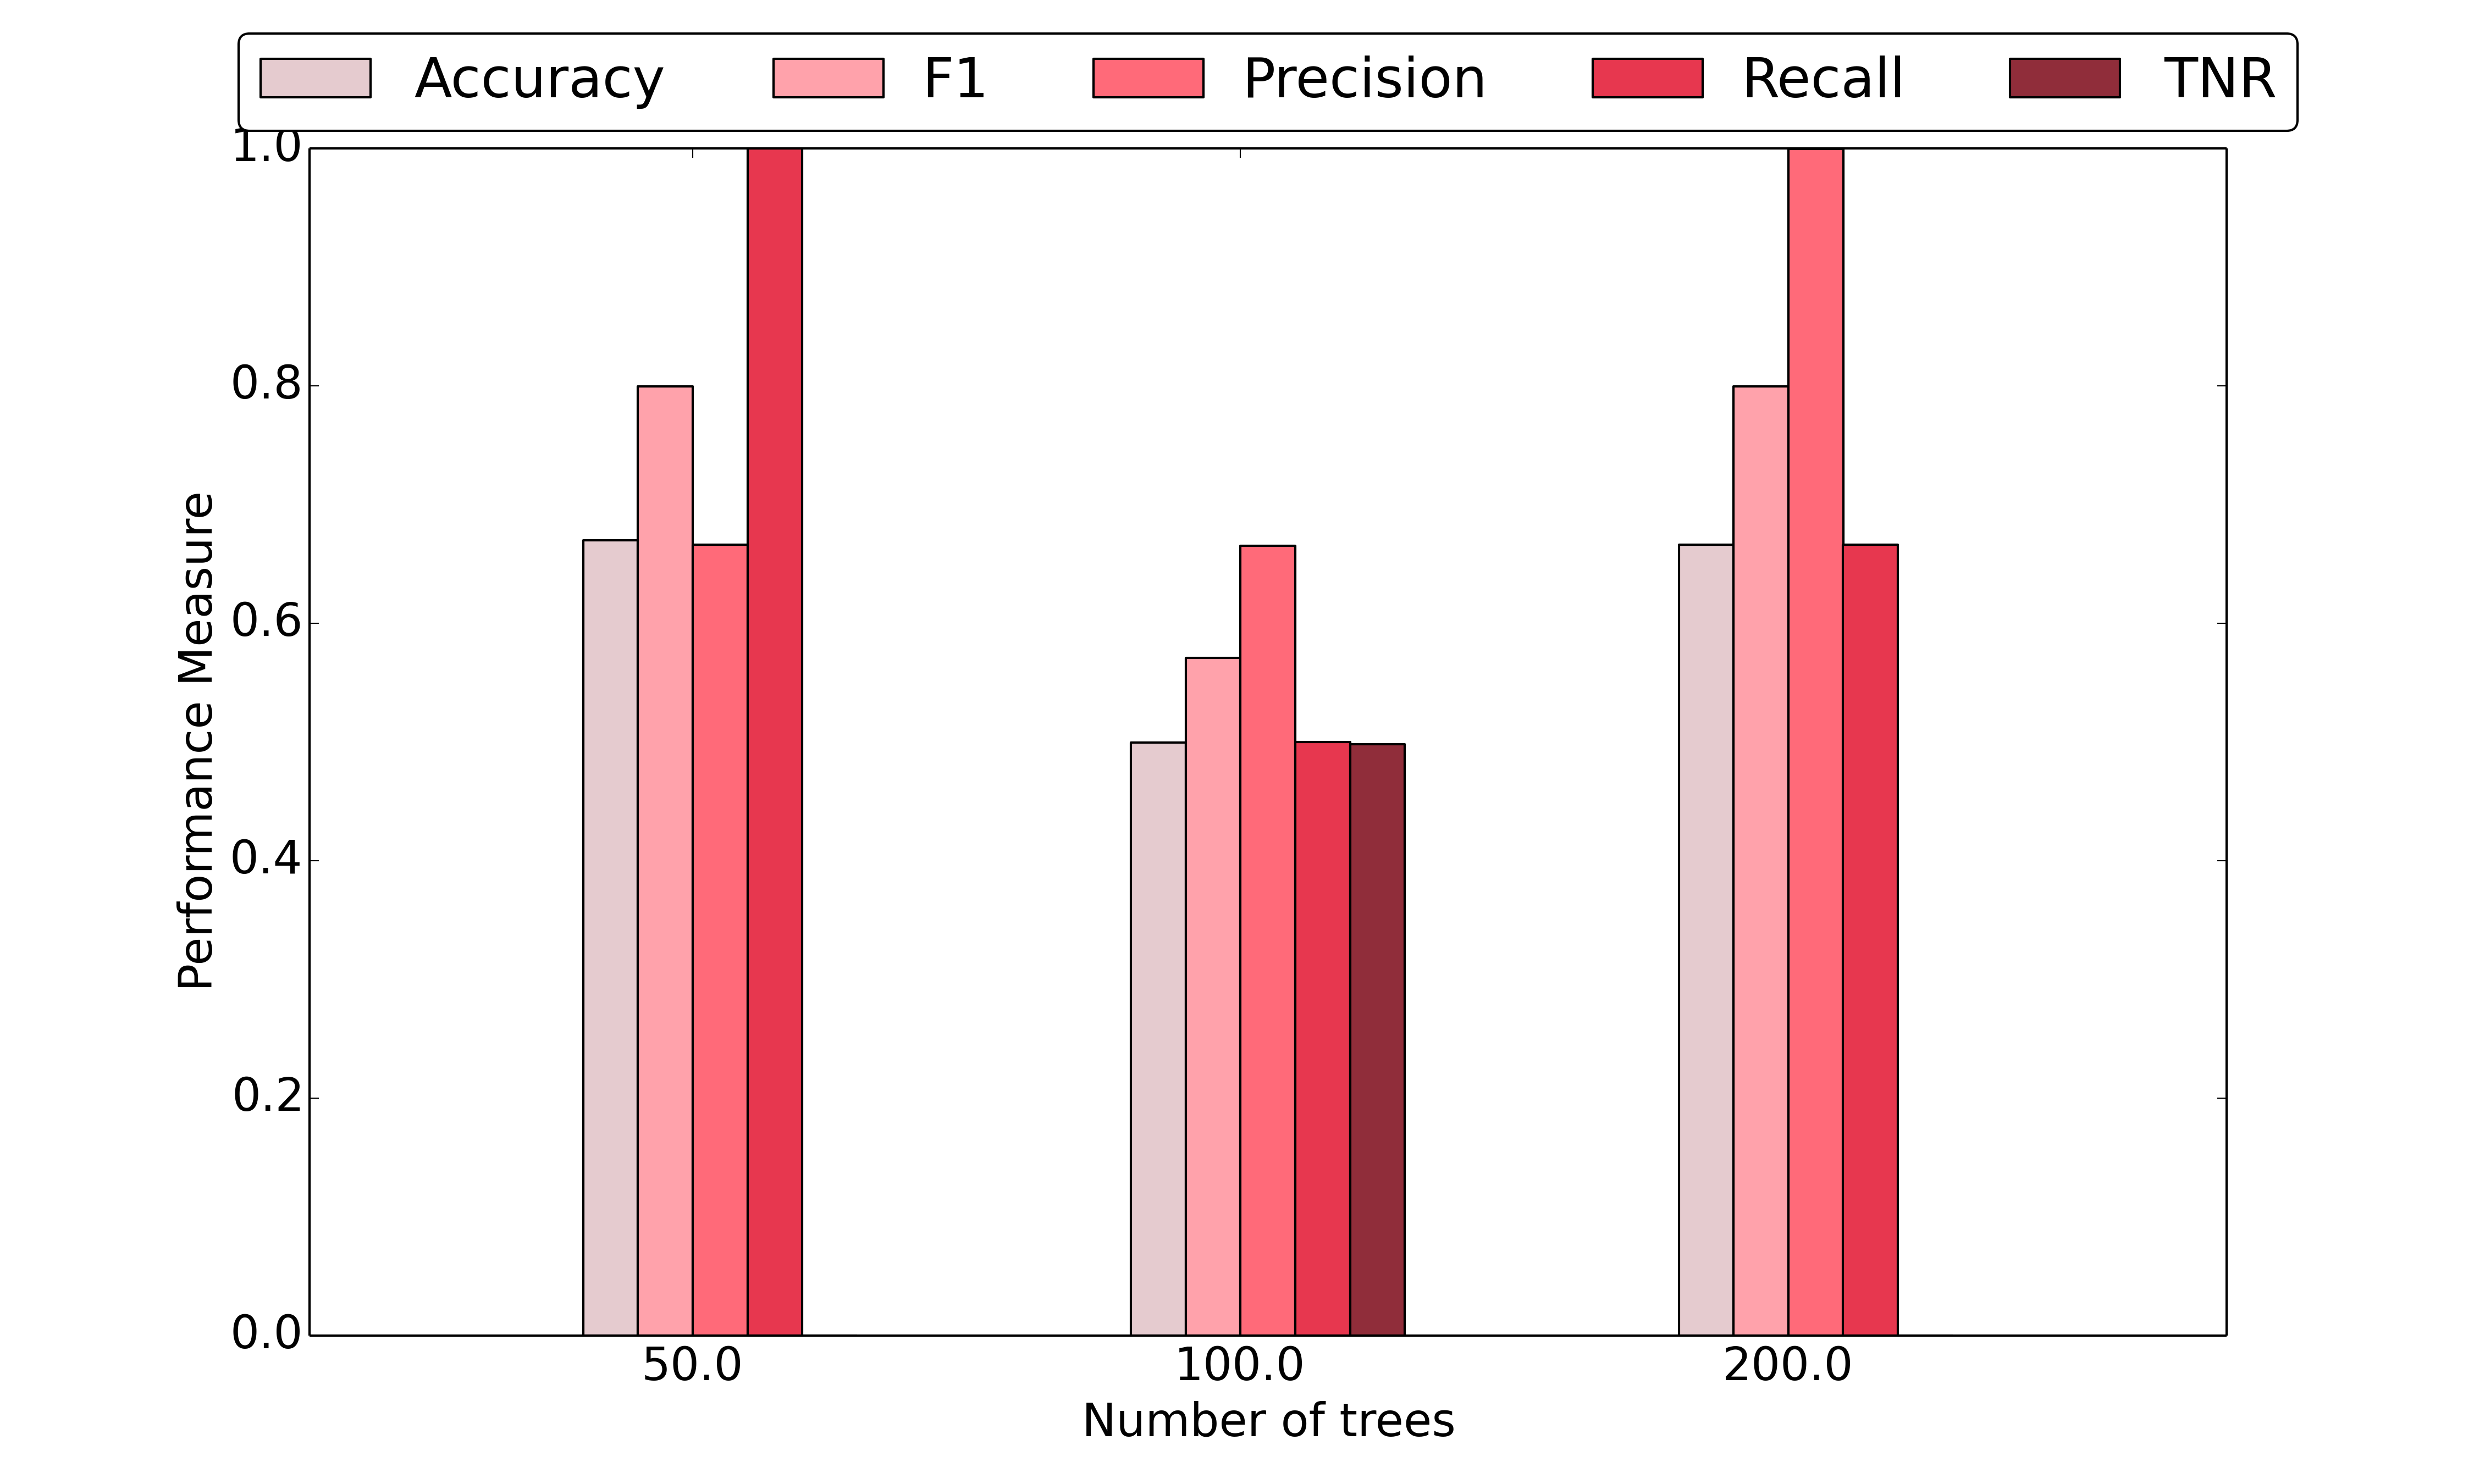
\includegraphics[scale=0.2]{figures/8Map-localLabelPerf.png}
\caption{\textit{Local-Label data} performance with trees in ${50,100,200}$.}
\end{subfigure}
\begin{subfigure}{.4\textwidth}
\centering
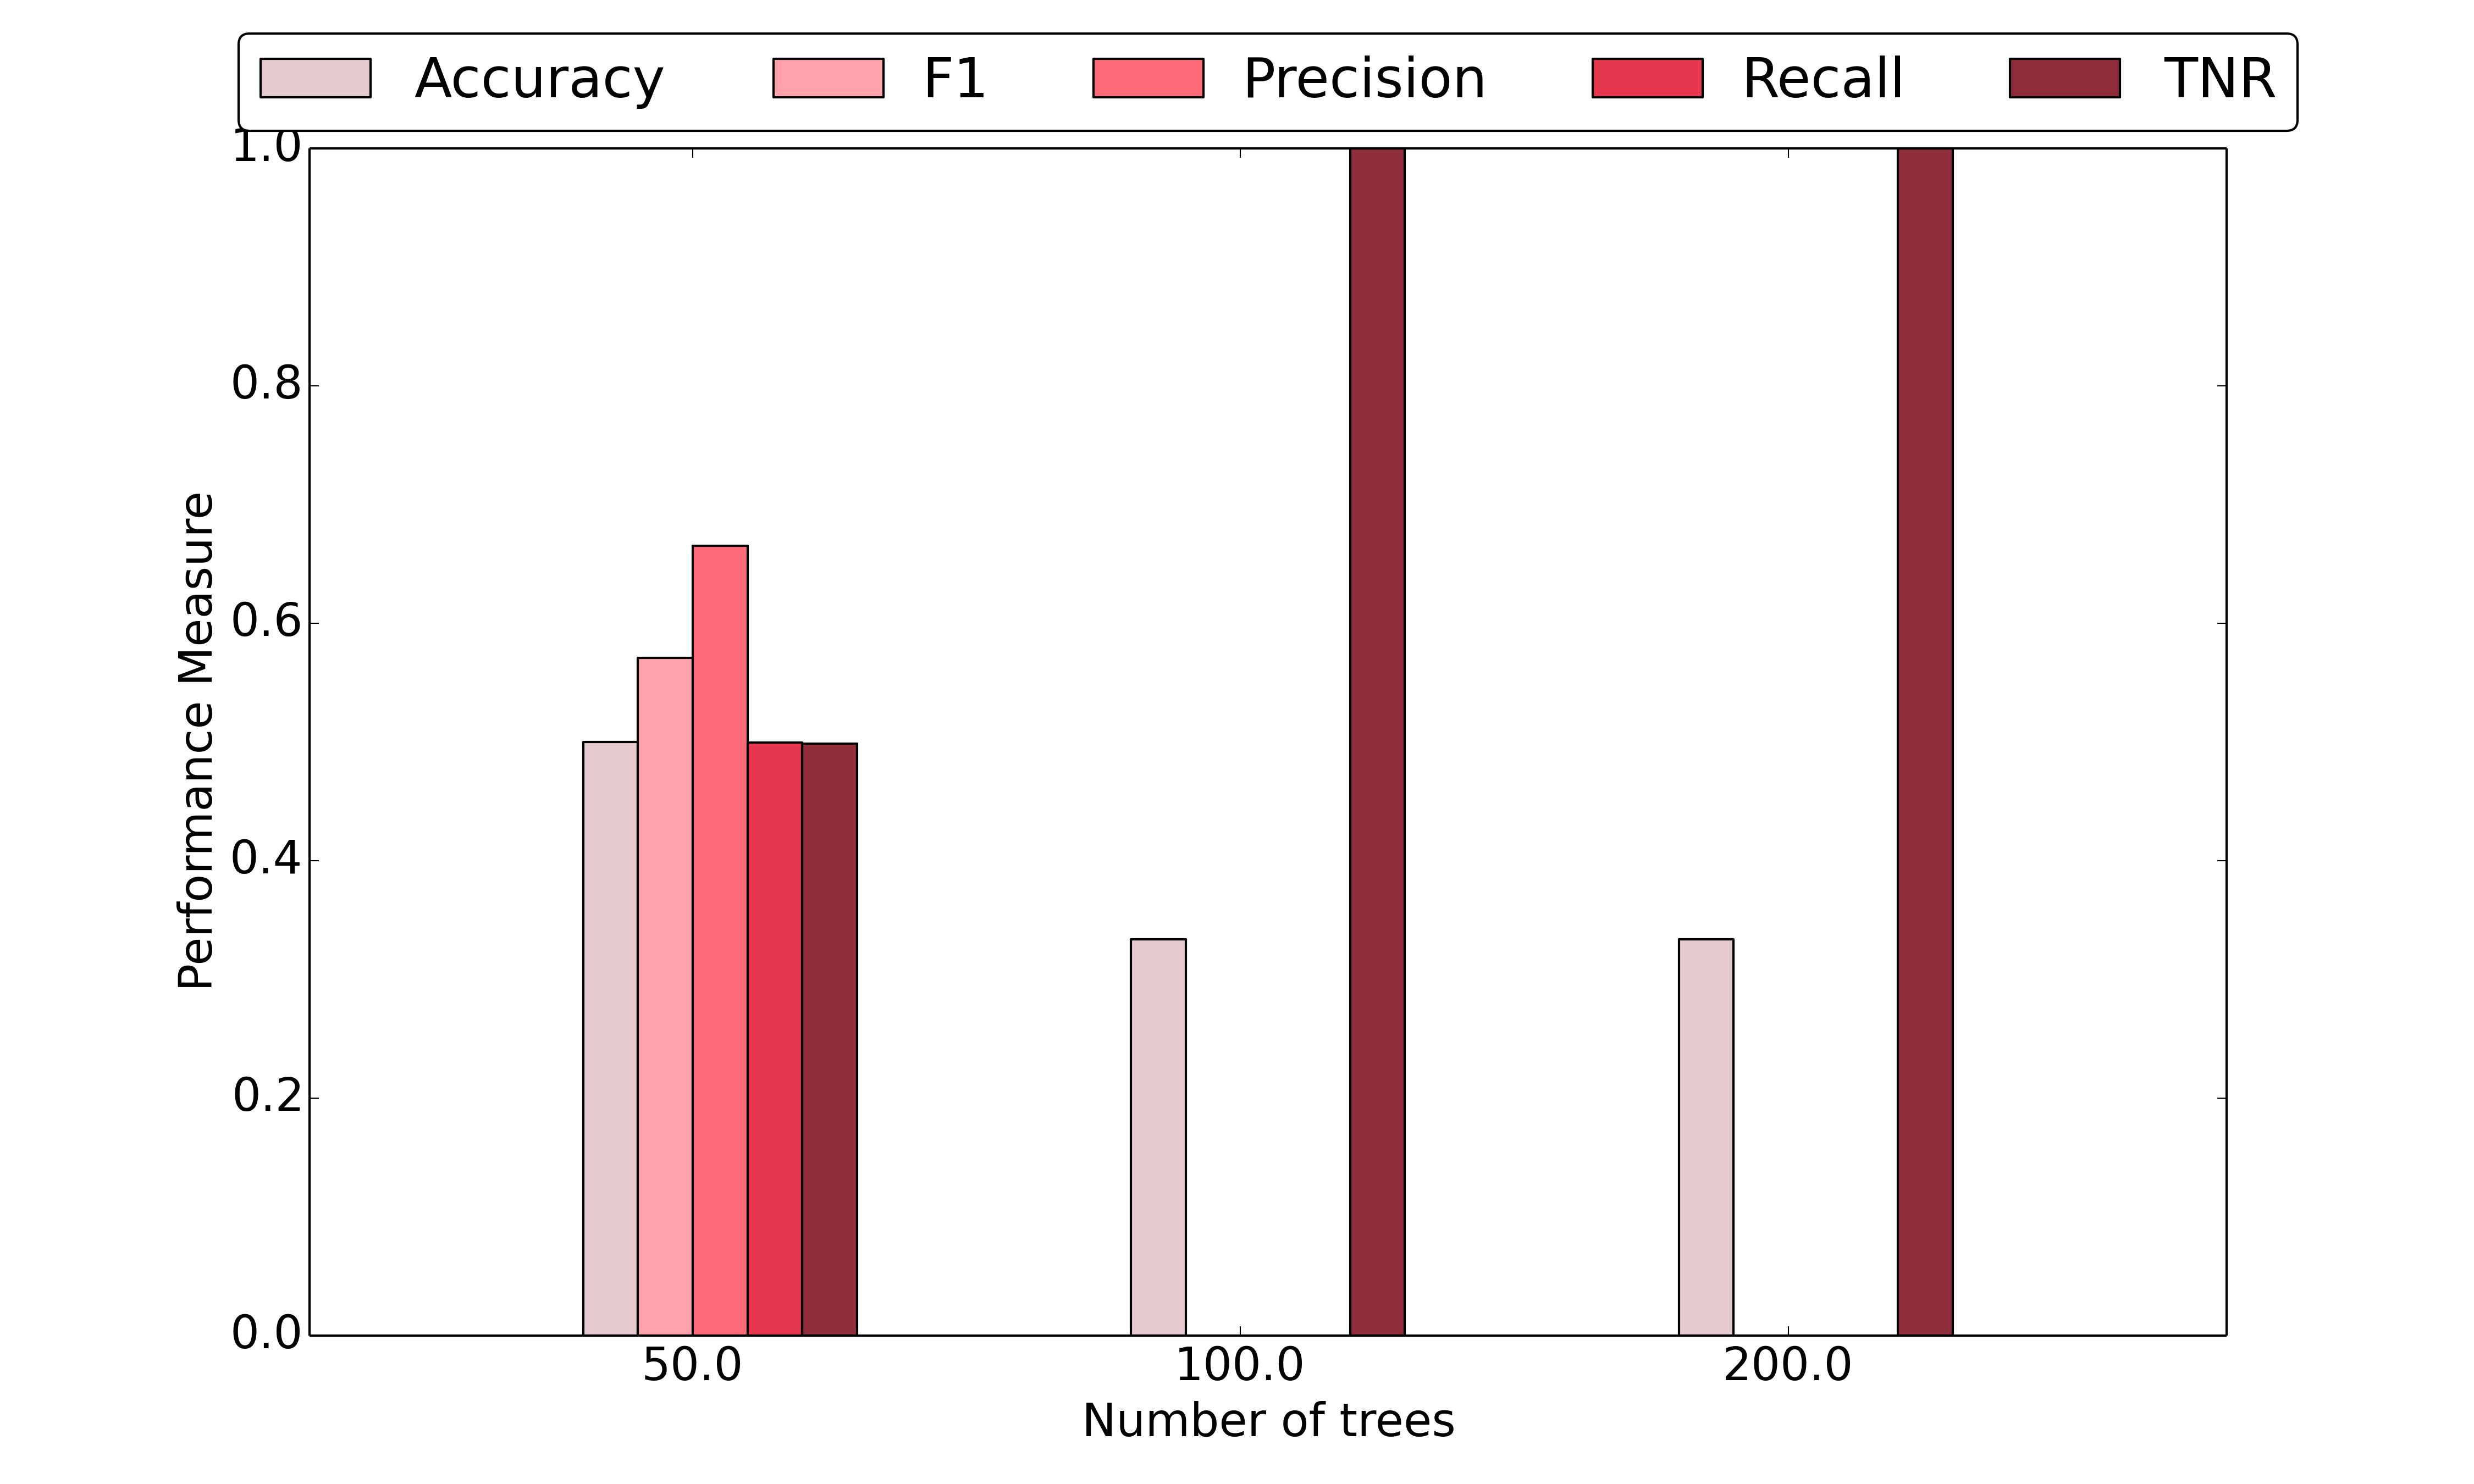
\includegraphics[scale=0.2]{figures/8Map-localFeatureLabelPerf.png}
\caption{\textit{Local-Feature-Label data} performance with trees in ${50,100,200}$.}
\end{subfigure}
\begin{subfigure}{.4\textwidth}
\centering
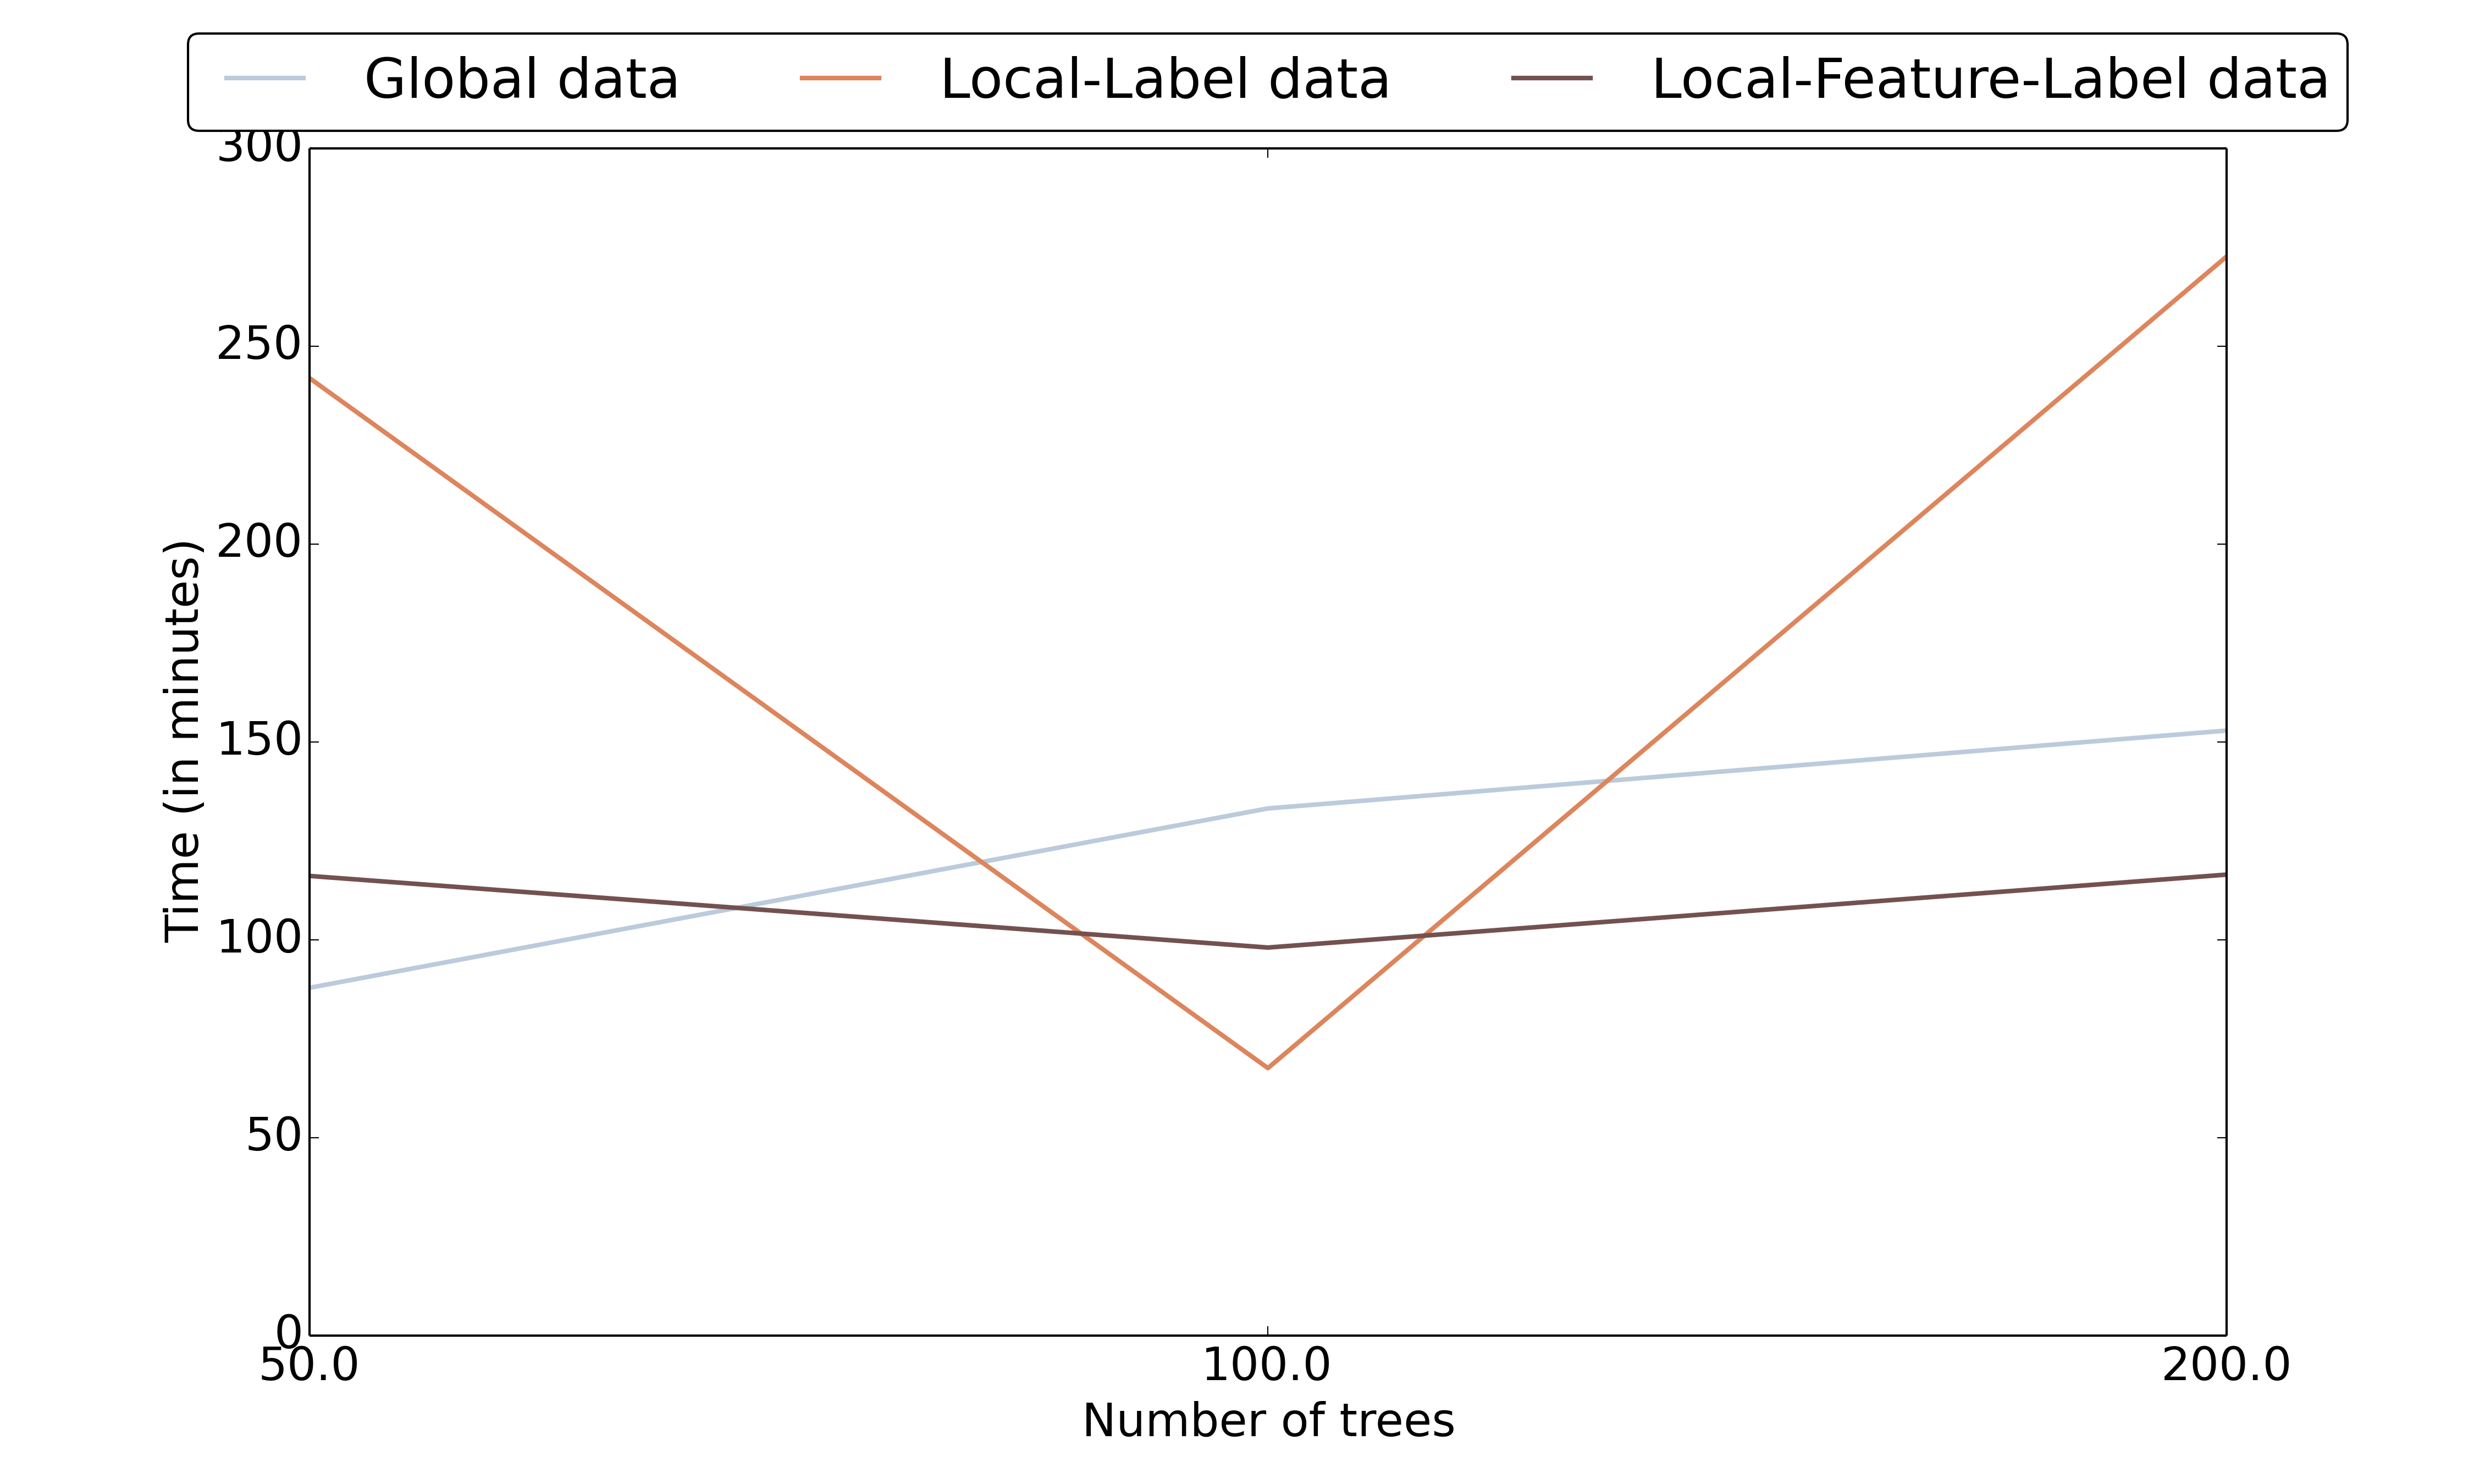
\includegraphics[scale=0.2]{figures/8MapperTime.png}
\caption{Time taken to construct corresponding trees in all corresponding experiments.}
\end{subfigure}
\caption{\textit{Harp}-based parallel code's performance with 8 mappers - \textit{Truly Global models}.}
\label{fig:trulyGlobalModels}
\end{figure*}

\begin{figure*}[t]
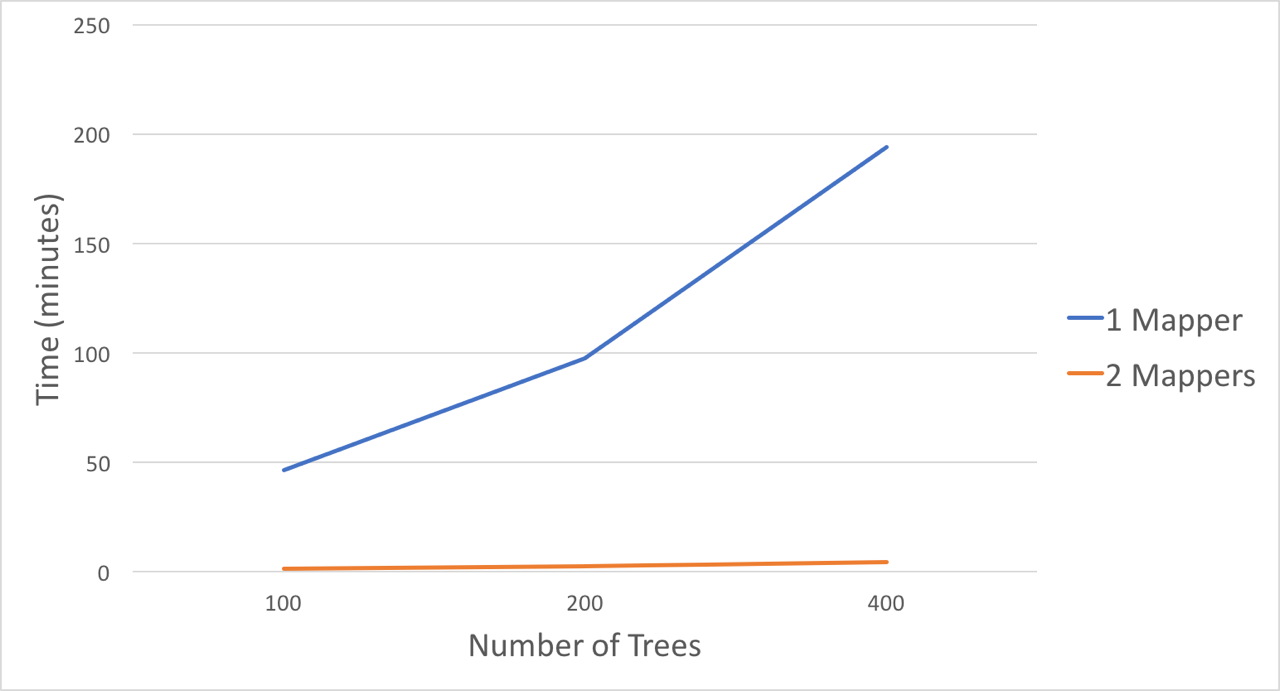
\includegraphics[scale=0.5]{figures/TimeRatioAnalysis.png}
\centering
\caption{Time Ratio Analysis between 1 mapper and 2 mappers as a function of global number of trees.}
\label{fig:timeRatio}
\end{figure*}

\textbf{Approximate global model experiments:} We next experimented with 2 mappers due to the following reasons: (1) due to resource limitations on our local machine to handle 8 mappers - context switching overhead would act opposite to the the efficacy gained from parallelization, and hence, would not lead to a gain, (2) random forests are known to be low bias, high variance classifiers - while, with parallelization, huge forests can be learned efficiently, this does not necessarily improve the classifier, as it increases variance of prediction due to the high number of trees, and (3) to study the trade-off between utilizing all the distributed data (as used in \textit{Truly Global models} with 8 mappers) to utilizing most of the distributed data from the representative locations (as utilized by the 2 mappers here). The results w.r.t. these experiments are shown in Figure \ref{fig:approximateGlobalModels}. It can be seen that computation time with \textit{Global data} increases with more trees, more rapidly than the other two \textit{Local data} models (specifically \textit{Local-Feature-Label data}. This is because the distribution of data in the global case is a mixture of the various local distributions, making it harder for feature selection or tree construction during learning. But correspondingly, it can also be seen that the model's learned from the \textit{Global data} are better than the \textit{Local-Feature-Label data} models, as expected. Therefore, this trade-off is crucial in real-time decisions of viable model construction vs. minimal computational overhead. Surprisingly, \textit{Local-Label data} performs really well; this may be because the trees learned are highly effective at modeling the designated label distributions locally, leading to low variance models on the global scale (while maintaining low bias). But it must be noted that this data is generated artificially, and seldom do such useful scenarios surface in real distributed data.

\textbf{Truly global model experiments: } In these experiments we used \textit{8 Mappers} to learn Radnom Forests of size 400, 800, and 1600  (50, 100, and 200 per mapper). As expected with more number of trees, the performance began to degrade as Random Forests fit to the bias in the data, essentially predicting the majority class found at the mappers. This is characteristic of the dataset, and not of the distributed method. Another peculiar behavior due to the random bootstrapping is the convergence of the trees being learned - hence the peculiar hinge in the behavior of \textit{Local-label data}. But this is a characteristic of random forest classifiers. Although the performance of Random Forest learned with 8 mappers is very low, it is important to remember that a large proportion of the datapoints used to learn the 8 Mapper models had missing heart-rate feature values.  This likely, highly impacted the performance of the classifier, as the test-set had the feature present. Due to the high proportion of missing data the train data here may have been sub-optimal . This is compounded by the fact that these forests are likely to have overfitted this suboptimal data (high number of tress $\rightarrow$ overfit model) causing the \textit{Truly Global models} to be worse than the \textit{Approximately Global models}.

\textbf{Time Ratio Analysis: } As can be seen in \ref{fig:timeRatio}, scaling up the number of mappers does not negatively impact the amount of time it takes to learn Random Forests of sizes 100, 200, and 400. In fact, scaling up our number of mappers significantly decreases the run-time of learning each forest. Therefore, our distributed approach to learning random forests is efficient and beneficial. Additionally, as can be seen form the results discussed above, so long as the number of trees is not grown to a massive amount (more than 400 for this dataset), learning random forests with our distributed implementation produces good random forest models in a minimal amount of time.


\section{Conclusions}
Random Forests in literature have been proven to be low bias, high variance classifiers. Although their learning principle is random, they have been shown to have high empirical performance. Their natural structure is amenable to parallel programming making it a rich option for modeling distributed data. Therefore, here we tested how well a Random Forest performs in a distributed environment by modeling data of different characteristics, and the corresponding effects they have on the performance of Random Forests. From our analysis, we conclude that Random Forests are effective if trained on at least a subset of the global data , as opposed to completely localized data, as the latter seems to restrict the models highly - inducing bias. Interestingly, utilizing the complete global data for training Random Forests can lead to high variance behavior as well. Therefore, moving forward, it would be interesting to explore the degree of \textit{``data globalization"} necessary to create effective Random Forests.

\section{Acknowledgments}
From our experiments and analysis in this term project we have learned to utilize the Harp infrastructure effectively (and a little efficiently). Towards this, we are highly thankful to Ethan Li and Bingjing Zhang for their continued patience and crucial help. To Prof. Bo Peng for his insightful comments during the execution of the project and structured advice for organizing the experiments. And of course, to Prof. Judy Qui for her constant support, her encouraging classes, and friendly nature. 

\bibliographystyle{abbrv}
\bibliography{paper}  
\end{document}